%%%%%%%%%%%%%%%%  NUMERICAL RESULTS %%%%%%%%%%%%%%%%%%%%%
\chapter{Numerical Results} \thispagestyle{chapterpage}
\label{chapter:numerical_results}

\todoinline{Run tests with lower tolerance. Might favor Newton/JTR}

Reservoir simulation packages are large and complex programs since input of well specifications, grid parameters, fluid definitions, etc., must be supported by the code base, along with all kinds of utility functions. In order to test the numerical methods described in Chapter \ref{chapter:numerical_methods} we use the open source simulator supplied by the Open Porous Media initiative, or \opm, see \citet{opm_2014}. Section \ref{section:opm_package} starts this chapter with a brief overview of the \opm transport solver classes used as a basis for the new root finder implementations (see Section \ref{section:root_finders}). Section \ref{section:test_cases} presents a number of tests cases and the corresponding numerical results from running the cases with the root finders from Section \ref{section:root_finders}.

%%%%%%%%%%%%%%%%  THE OPM PACKAGE %%%%%%%%%%%%%%%%%%%%%
\section{The OPM Package}
\label{section:opm_package}
\todoinline{Fix the over/underfull lines}
The \opm package provides a range of modules for grid handling, polymer injection, upscaling methods, and more. The \code{opm-core} module contains basic grid and well handling, and IO utilities, along with pressure and transport solvers for solving the porous media fluid flow problems described in Section \ref{section:fluid_models}. In fact, the \opm package implements the exact numerical methods described in Section \ref{section:seq_splitting_method} through the \code{Opm::IncompTpfa} pressure solver and the \code{Opm::TransportSolverTwophaseReorder} transport solver classes using the Regula Falsi, see Section \ref{section:regula_falsi}, for the single cell problems resulting from  reordering as described in Section \ref{section:reordering}. Listings \ref{listing:test_driver_2D} and \ref{listing:test_driver_3D} show the code for the driver programs implementing the sequential splitting scheme using the \opm library. The class \code{Opm::TransportSolverTwophaseReorder} implements the functionality for solving the residual equations in Equation (\ref{eq:residual_two_phase_transport}) and (\ref{eq:residual_two_phase_transport_gravity}) and is instantiated with the static properties of the simulation, such as the grid specification and fluid model. At each iteration of the sequential splitting method, as outlined in Algorithm \ref{algorithm:sequential_splitting}, a new saturation field is computed by calling the method \code{solve(\dots)} on a \code{Opm::TransportSolverTwophaseReorder} object. The arguments to the solve method includes the time step $\Delta t$, and an instance of the fluid state class \code{TwophaseState} containing the saturation, flux, and other state information for every cell $V \in \mathcal{T}$. The \code{solve} method proceeds to computes the ordering of the flux graph based on the flux values obtained by solving the pressure equation. This ordering leads to a set of pseudo cells consisting of one or more regular cells, as described in Section \ref{section:reordering}. The new saturation field is finally obtained by iterating over all the pseudo cells and solving each subproblem by either the single cell root finders or the multi cell solver depending on the number of grid cells in each pseudo cell. The single cell root finders are the main focus of this work. The transport equation residuals are implemented by two structs, Equation (\ref{eq:residual_two_phase_transport}) in the struct \code{Residual} and Equation (\ref{eq:residual_two_phase_transport_gravity}) in the struct \code{GravityResidual}. These structs are supplied with an ()-operator taking the update saturation $S_V^{n+1}$ as an argument and returning the residual value.
\begin{figure}[ht]%
\centering%
\tikzsetnextfilename{spe10_perm_tarbert}
\begin{subfigure}[b]{0.49\textwidth}%
\centering%
\begin{tikzpicture}%
    \node[anchor=south west,inner sep=0] (image) at (0,0) {\includegraphics[width=\textwidth]{figures/spe10_tarbert_view.eps}};%
\end{tikzpicture}%
\caption{Top view}%
\label{fig:tarbert}%
\end{subfigure}%
\centering%
\tikzsetnextfilename{spe10_perm_upperness}
\begin{subfigure}[b]{0.49\textwidth}%
\centering%
\begin{tikzpicture}%
    \node[anchor=south west,inner sep=0] (image) at (0,0) {\includegraphics[width=\textwidth]{figures/spe10_upperness_view.eps}};%
\end{tikzpicture}%
\caption{Bottom view}%
\label{fig:upper_ness}%
\end{subfigure}%
\caption{Inhomogeneous permeability data from the second SPE10 data set \citep{spe10_2000}. The top 35 layers are part of the Tarbert formation. The lower 50 are part of the Upper Ness formation. The model dimension is  $\unit[1200]{ft} \times \unit[2200]{ft} \times \unit[170]{ft}$, approximately $\unit[335]{m} \times \unit[670]{m} \times \unit[52]{m}$, with $60\times220\times85$ cells.}%
\label{fig:spe10_perm}%
\end{figure}

%%%%%%%%%%%%  TEST CASES  %%%%%%%%%%
\section{Test Cases}
\label{section:test_cases}
%%%%%%%%%%%%  TEST PROCEDURE  %%%%%%%%%%
\subsection{Test Procedure}
\label{section:test_procedure}
In order to test the efficiency of the single cell solvers the \opm library was installed on a server with Intel\textregistered{}  Xeon\textregistered{}  X7542 CPUs running at \unit[2.67]{GHz} with a \unit[18432]{kB} cache size. The server has \unit[252]{GB} of available ram. The homogeneous tests have been run using the C++ driver program included in Listing \ref{listing:test_driver_2D}. For the inhomogeneous tests the code in Listing \ref{listing:test_driver_3D} was used. Further, all test cases were checked against the reference Regula Falsi solver, see Section \ref{section:regula_falsi}, to ensure that the correct solution is found. The iteration count for each solver was reported along with the solution updates to determine the convergence speed versus iteration for each method. Finally, the total CPU time is reported to check the overall performance of each root finder. In the following we will test these methods for solving the single cell residual: Brent (B), Section \ref{section:brents_method}, Regula Falsi (RF), Section \ref{section:regula_falsi}, Ridders (R), Section \ref{section:ridders_method}, and the Approximate (TR*) and Precise (TR) Trust Region methods, Section \ref{section:trust_regions}. The method name abbreviations in the parentheses will be used in the following.

%%%%%%%%%%%%  QUARTER FIVE SPOT %%%%%%%%%%
\subsection{Case A: Quarter Five Spot}
\label{section:caseA}
\todoinline{Error plot against reference solver for hom. Q5}
The \emph{quarter five spot}, abbreviated Q5, is a quadratic 2D domain with a source in one corner and a sink in the opposite corner along the diagonal. Here the cells in the domain have dimensions $\unit[10]{m}\times\unit[10]{m}\times\unit[10]{m}$. The fluid density is set to $\unitfrac[1000]{kg}{m^3}$, porosity $\unit[0.5]{}$ and the formation has homogeneous permeability $\unit[10]{mD}$. The simulation is run on a $20\times 20$ grid with a source in one corner cell and a sink in the diagonally opposite corner, both of magnitude $\unitfrac[50]{m^3}{s}$. The viscosity is varied through three cases; $\mu_w = \unit[1]{cP}$ and $\mu_o= \unit[1]{cP}$, $\mu_w = \unit[1]{cP}$ and $\mu_o= \unit[10]{cP}$, and $\mu_w = \unit[10]{cP}$ and $\mu_o= \unit[1]{cP}$. Figure \ref{fig:sat_hist_hom} shows an example of an advancing saturation profile from a simulation of the homogeneous Q5 problem. Because of the uniform permeability and the quadratic geometry the saturation profile is symmetric around the diagonal between the source and sink.
\tikzsetnextfilename{sat_hist_hom}
\begin{figure}[ht]
\centering
\begin{tikzpicture}
    \node[anchor=south west,inner sep=0] (image) at (0,0) {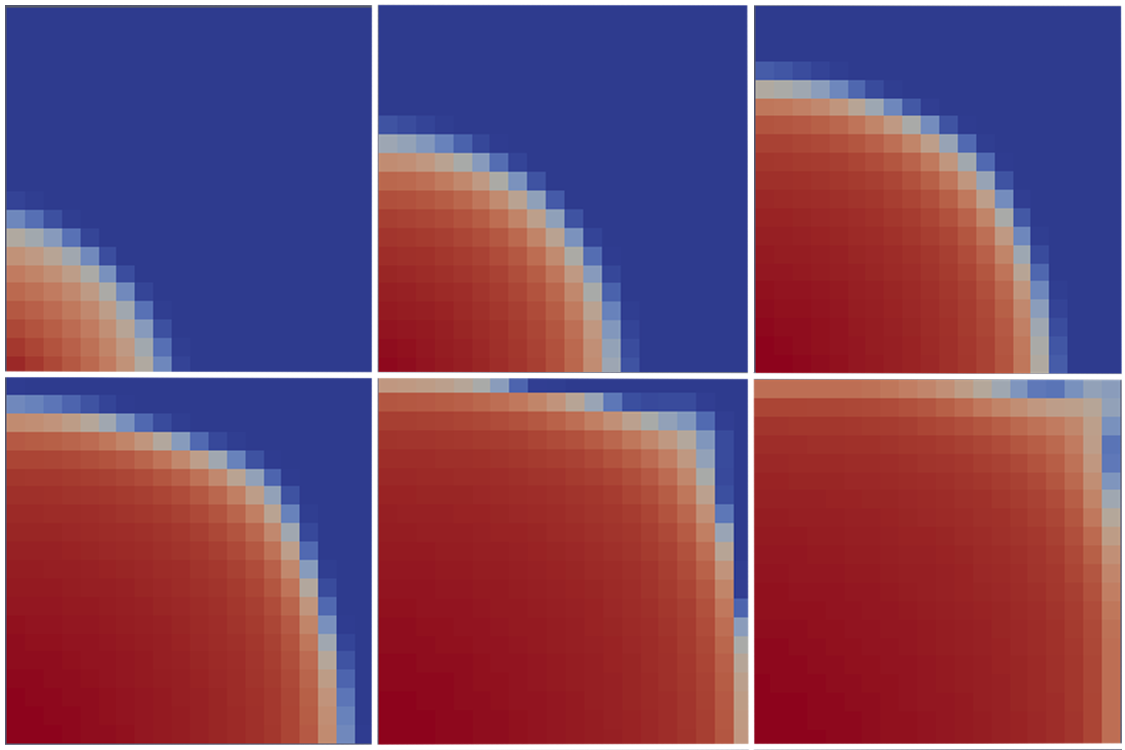
\includegraphics[width=0.6\textwidth]{figures/sat-hist-s-i-T-300-t-30-perm-10.png}};
\end{tikzpicture}
\caption{$S_w$ profile when solving the Q5 problem on a 20x20 grid with $t_{\text{end}} = \unit[300]{d}$ and $\Delta t = \unit[60]{d}$. The region has a homogeneous permeability of $\unit[10]{mD}$. Blue is oil, red is water.}
\label{fig:sat_hist_hom}
\end{figure}

%%%%% 120 by 120 %%%%%%%
\subsubsection{120 m by 120 m comments}
The total iteration count spent when solving the Q5 problem is presented in Figures \ref{fig:q5_iterations_perm_h_10_i_180} and \ref{fig:q5_cputime_perm_h_10_i_180} for all root finders. We include the viscosity ratio because of the significant influence it has on the shape of $f_w$, as indicated by Figure \ref{fig:fractional_flow_wrt_viscosity_ratio}. The trend in the data is that Brent's method uses the highest number of iterations, while the precise trust region scheme needs significantly fewer iterations than all other methods. The data also indicates that the average iteration count is lower and the differences between the methods are smaller for larger values of $M$.
\begin{figure}[!ht]
\tikzsetnextfilename{q5_iterations_perm_h_10_m_1_10_i_180_dt_1to30}
\begin{subfigure}[b]{0.49\textwidth} %%%%%%%%%%% M = 0.1 %%%%%%%%%%%%%%
\begin{tikzpicture}
    \pgfplotstablegetrowsof{datafiles/q5-iterations-s-r-T-300-m-1-10-dim-120-120-20-20-perm-h-10-i-180.data}
    \pgfmathsetmacro\yfin{\pgfmathresult}
    \pgfmathsetmacro\yini{5}
    \begin{semilogyaxis}[
            width=0.97\textwidth,
            height=0.26\textheight,
            ymin=9999,
            ymax=600000,
            xlabel={dt~[d]},
            ylabel={\#iterations},
            grid=both,
            skip coords between index={\yini}{\yfin}
            ]
        \addplot table[col sep=comma, trim cells=true,x=dt, y=iterations] {datafiles/q5-iterations-s-r-T-300-m-1-10-dim-120-120-20-20-perm-h-10-i-180.data};
        \addplot table[col sep=comma, trim cells=true,x=dt, y=iterations] {datafiles/q5-iterations-s-t-T-300-m-1-10-dim-120-120-20-20-perm-h-10-i-180.data};
        \addplot table[col sep=comma, trim cells=true,x=dt, y=iterations] {datafiles/q5-iterations-s-a-T-300-m-1-10-dim-120-120-20-20-perm-h-10-i-180.data};
        \addplot table[col sep=comma, trim cells=true,x=dt, y=iterations] {datafiles/q5-iterations-s-b-T-300-m-1-10-dim-120-120-20-20-perm-h-10-i-180.data};
        \addplot table[col sep=comma, trim cells=true,x=dt, y=iterations] {datafiles/q5-iterations-s-i-T-300-m-1-10-dim-120-120-20-20-perm-h-10-i-180.data};
        \legend{RF,TR,TR*,B,R}
    \end{semilogyaxis}
\end{tikzpicture}%
\caption{$M =0.1$} \label{fig:q5_iterations_perm_h_10_m_1_10_i_180_dt_1to30}
\end{subfigure}%
~
\tikzsetnextfilename{q5_iterations_perm_h_10_m_1_10_i_180_dt_40to150}
\begin{subfigure}[b]{0.49\textwidth}
\begin{tikzpicture}
    \pgfplotstablegetrowsof{datafiles/q5-iterations-s-r-T-300-m-1-10-dim-120-120-20-20-perm-h-10-i-180.data}
    \pgfmathsetmacro\yfin{5}
    \pgfmathsetmacro\yini{0}
    \begin{semilogyaxis}[
            width=0.97\textwidth,
            height=0.26\textheight,
            ymin=999,
            ymax=20000,
            xlabel={dt~[d]},
            ylabel={\#iterations},
            grid=both,
            skip coords between index={\yini}{\yfin}
            ]
        \addplot table[col sep=comma, trim cells=true,x=dt, y=iterations] {datafiles/q5-iterations-s-r-T-300-m-1-10-dim-120-120-20-20-perm-h-10-i-180.data};
        \addplot table[col sep=comma, trim cells=true,x=dt, y=iterations] {datafiles/q5-iterations-s-t-T-300-m-1-10-dim-120-120-20-20-perm-h-10-i-180.data};
        \addplot table[col sep=comma, trim cells=true,x=dt, y=iterations] {datafiles/q5-iterations-s-a-T-300-m-1-10-dim-120-120-20-20-perm-h-10-i-180.data};
        \addplot table[col sep=comma, trim cells=true,x=dt, y=iterations] {datafiles/q5-iterations-s-b-T-300-m-1-10-dim-120-120-20-20-perm-h-10-i-180.data};
        \addplot table[col sep=comma, trim cells=true,x=dt, y=iterations] {datafiles/q5-iterations-s-i-T-300-m-1-10-dim-120-120-20-20-perm-h-10-i-180.data};
        %\legend{RF,TR,TR*,B,R}
    \end{semilogyaxis}
\end{tikzpicture}%
\caption{$M =0.1$} \label{fig:q5_iterations_perm_h_10_m_1_10_i_180_dt_40to150}
\end{subfigure}%
\vspace{0.3cm} %%%%%%%%%%% M = 1 %%%%%%%%%%%%%%
\tikzsetnextfilename{q5_iterations_perm_h_10_m_1_1_i_180_dt_1to30}
\begin{subfigure}[b]{0.49\textwidth}
\begin{tikzpicture}
    \pgfplotstablegetrowsof{datafiles/q5-iterations-s-r-T-300-m-1-10-dim-120-120-20-20-perm-h-10-i-180.data}
    \pgfmathsetmacro\yfin{\pgfmathresult}
    \pgfmathsetmacro\yini{5}
    \begin{semilogyaxis}[
            width=0.97\textwidth,
            height=0.26\textheight,
            ymin=9999,
            ymax=600000,
            xlabel={dt~[d]},
            ylabel={\#iterations},
            grid=both,
            skip coords between index={\yini}{\yfin}
            ]
         \addplot table[col sep=comma, trim cells=true,x=dt, y=iterations] {datafiles/q5-iterations-s-r-T-300-m-1-1-dim-120-120-20-20-perm-h-10-i-180.data};
        \addplot table[col sep=comma, trim cells=true,x=dt, y=iterations] {datafiles/q5-iterations-s-t-T-300-m-1-1-dim-120-120-20-20-perm-h-10-i-180.data};
        \addplot table[col sep=comma, trim cells=true,x=dt, y=iterations] {datafiles/q5-iterations-s-a-T-300-m-1-1-dim-120-120-20-20-perm-h-10-i-180.data};
        \addplot table[col sep=comma, trim cells=true,x=dt, y=iterations] {datafiles/q5-iterations-s-b-T-300-m-1-1-dim-120-120-20-20-perm-h-10-i-180.data};
        \addplot table[col sep=comma, trim cells=true,x=dt, y=iterations] {datafiles/q5-iterations-s-i-T-300-m-1-1-dim-120-120-20-20-perm-h-10-i-180.data};
        \legend{RF,TR,TR*,B,R}
    \end{semilogyaxis}
\end{tikzpicture}%
\caption{$M =1$} \label{fig:q5_iterations_perm_h_10_m_1_1_i_180_dt_1to30}
\end{subfigure}%
~
\tikzsetnextfilename{q5_iterations_perm_h_10_m_1_1_i_180_dt_40to150}
\begin{subfigure}[b]{0.49\textwidth}
\begin{tikzpicture}
    \pgfplotstablegetrowsof{datafiles/q5-iterations-s-r-T-300-m-1-10-dim-120-120-20-20-perm-h-10-i-180.data}
    \pgfmathsetmacro\yfin{5}
    \pgfmathsetmacro\yini{0}
    \begin{semilogyaxis}[
            width=0.97\textwidth,
            height=0.26\textheight,
            ymin=999,
            ymax=20000,
            xlabel={dt~[d]},
            ylabel={\#iterations},
            grid=both,
            skip coords between index={\yini}{\yfin}
            ]
         \addplot table[col sep=comma, trim cells=true,x=dt, y=iterations] {datafiles/q5-iterations-s-r-T-300-m-1-1-dim-120-120-20-20-perm-h-10-i-180.data};
        \addplot table[col sep=comma, trim cells=true,x=dt, y=iterations] {datafiles/q5-iterations-s-t-T-300-m-1-1-dim-120-120-20-20-perm-h-10-i-180.data};
        \addplot table[col sep=comma, trim cells=true,x=dt, y=iterations] {datafiles/q5-iterations-s-a-T-300-m-1-1-dim-120-120-20-20-perm-h-10-i-180.data};
        \addplot table[col sep=comma, trim cells=true,x=dt, y=iterations] {datafiles/q5-iterations-s-b-T-300-m-1-1-dim-120-120-20-20-perm-h-10-i-180.data};
        \addplot table[col sep=comma, trim cells=true,x=dt, y=iterations] {datafiles/q5-iterations-s-i-T-300-m-1-1-dim-120-120-20-20-perm-h-10-i-180.data};
        %\legend{RF,TR,TR*,B,R}
    \end{semilogyaxis}
\end{tikzpicture}%
\caption{$M =1$} \label{fig:q5_iterations_perm_h_10_m_1_1_i_180_dt_40to150}
\end{subfigure}%
\vspace{0.3cm} %%%%%%%%%%% M = 10 %%%%%%%%%%%%%%
\tikzsetnextfilename{q5_iterations_perm_h_10_m_10_1_i_180_dt_1to30}
\begin{subfigure}[b]{0.49\textwidth}
\begin{tikzpicture}
    \pgfplotstablegetrowsof{datafiles/q5-iterations-s-r-T-300-m-1-10-dim-120-120-20-20-perm-h-10-i-180.data}
    \pgfmathsetmacro\yfin{\pgfmathresult}
    \pgfmathsetmacro\yini{5}
    \begin{semilogyaxis}[
            width=0.97\textwidth,
            height=0.26\textheight,
            ymin=8000,
            ymax=600000,
            xlabel={dt~[d]},
            ylabel={\#iterations},
            grid=both,
            skip coords between index={\yini}{\yfin}
            ]
         \addplot table[col sep=comma, trim cells=true,x=dt, y=iterations] {datafiles/q5-iterations-s-r-T-300-m-10-1-dim-120-120-20-20-perm-h-10-i-180.data};
        \addplot table[col sep=comma, trim cells=true,x=dt, y=iterations] {datafiles/q5-iterations-s-t-T-300-m-10-1-dim-120-120-20-20-perm-h-10-i-180.data};
        \addplot table[col sep=comma, trim cells=true,x=dt, y=iterations] {datafiles/q5-iterations-s-a-T-300-m-10-1-dim-120-120-20-20-perm-h-10-i-180.data};
        \addplot table[col sep=comma, trim cells=true,x=dt, y=iterations] {datafiles/q5-iterations-s-b-T-300-m-10-1-dim-120-120-20-20-perm-h-10-i-180.data};
        \addplot table[col sep=comma, trim cells=true,x=dt, y=iterations] {datafiles/q5-iterations-s-i-T-300-m-10-1-dim-120-120-20-20-perm-h-10-i-180.data};
        \legend{RF,TR,TR*,B,R}
    \end{semilogyaxis}
\end{tikzpicture}%
\caption{$M =10$} \label{fig:q5_iterations_perm_h_10_m_10_1_i_180_dt_1to30}
\end{subfigure}%
~
\tikzsetnextfilename{q5_iterations_perm_h_10_m_10_1_i_180_dt_40to150}
\begin{subfigure}[b]{0.49\textwidth}
\begin{tikzpicture}
    \pgfplotstablegetrowsof{datafiles/q5-iterations-s-r-T-300-m-1-10-dim-120-120-20-20-perm-h-10-i-180.data}
    \pgfmathsetmacro\yfin{5}
    \pgfmathsetmacro\yini{0}
    \begin{semilogyaxis}[
            width=0.97\textwidth,
            height=0.26\textheight,
            ymin=999,
            ymax=20000,
            xlabel={dt~[d]},
            ylabel={\#iterations},
            grid=both,
            skip coords between index={\yini}{\yfin}
            ]
         \addplot table[col sep=comma, trim cells=true,x=dt, y=iterations] {datafiles/q5-iterations-s-r-T-300-m-10-1-dim-120-120-20-20-perm-h-10-i-180.data};
        \addplot table[col sep=comma, trim cells=true,x=dt, y=iterations] {datafiles/q5-iterations-s-t-T-300-m-10-1-dim-120-120-20-20-perm-h-10-i-180.data};
        \addplot table[col sep=comma, trim cells=true,x=dt, y=iterations] {datafiles/q5-iterations-s-a-T-300-m-10-1-dim-120-120-20-20-perm-h-10-i-180.data};
        \addplot table[col sep=comma, trim cells=true,x=dt, y=iterations] {datafiles/q5-iterations-s-b-T-300-m-10-1-dim-120-120-20-20-perm-h-10-i-180.data};
        \addplot table[col sep=comma, trim cells=true,x=dt, y=iterations] {datafiles/q5-iterations-s-i-T-300-m-10-1-dim-120-120-20-20-perm-h-10-i-180.data};
        %\legend{RF,TR,TR*,B,R}
    \end{semilogyaxis}
\end{tikzpicture}%
\caption{$M =10$} \label{fig:q5_iterations_perm_h_10_m_10_1_i_180_dt_40to150}
\end{subfigure}%
\caption{\#iterations used to solve a modified Q5 problem, Section \ref{section:caseA}, for varying root finders, time steps and viscosity ratios. Note that $\unit[120]{m} \times \unit[120]{m}$ cells are used here.}
\label{fig:q5_iterations_perm_h_10_i_180}
\end{figure}%
%
%\begin{figure}[!ht]
%\centering
%\tikzsetnextfilename{q5_iterations_perm_h_10_m_1_10_i_180}
%\begin{subfigure}[b]{0.8\textwidth}
%\begin{tikzpicture}
%    \pgfplotstablegetrowsof{datafiles/q5-iterations-s-r-T-300-m-1-10-dim-120-120-20-20-perm-h-10-i-180.data}
%    \pgfmathsetmacro\yfin{\pgfmathresult - 4}
%    \pgfmathsetmacro\yini{0}
%    \begin{semilogyaxis}[
%            width=0.97\textwidth,
%            height=0.26\textheight,
%            ymin=1000,
%            ymax=1000000,
%            xlabel={dt~[d]},
%            ylabel={\#iterations},
%            grid=both,
%            ]
%        \addplot table[col sep=comma, trim cells=true,x=dt, y=iterations] {datafiles/q5-iterations-s-r-T-300-m-1-10-dim-120-120-20-20-perm-h-10-i-180.data};
%        \addplot table[col sep=comma, trim cells=true,x=dt, y=iterations] {datafiles/q5-iterations-s-t-T-300-m-1-10-dim-120-120-20-20-perm-h-10-i-180.data};
%        \addplot table[col sep=comma, trim cells=true,x=dt, y=iterations] {datafiles/q5-iterations-s-a-T-300-m-1-10-dim-120-120-20-20-perm-h-10-i-180.data};
%        \addplot table[col sep=comma, trim cells=true,x=dt, y=iterations] {datafiles/q5-iterations-s-b-T-300-m-1-10-dim-120-120-20-20-perm-h-10-i-180.data};
%        \addplot table[col sep=comma, trim cells=true,x=dt, y=iterations] {datafiles/q5-iterations-s-i-T-300-m-1-10-dim-120-120-20-20-perm-h-10-i-180.data};
%                %\addplot table[col sep=comma, trim cells=true,x=dt, y=iterations] {datafiles/q5-iterations-s-g-T-300-m-1-10-dim-120-120-20-20-perm-h-10-i-180.data};
%        \legend{RF,TR,TR*,B,R}
%    \end{semilogyaxis}
%\end{tikzpicture}%
%\caption{$M =0.1$} \label{fig:q5_iterations_perm_h_10_m_1_10_i_180}
%\end{subfigure}%
%\vspace{0.3cm}
%\centering
%\tikzsetnextfilename{q5_iterations_perm_h_10_m_1_1_i_180}
%\begin{subfigure}[b]{0.8\textwidth}
%\begin{tikzpicture}
%    \begin{semilogyaxis}[
%            width=0.97\textwidth,
%            height=0.26\textheight,
%            ymin=1000,
%            ymax=1000000,
%            xlabel={dt~[d]},
%            ylabel={\#iterations},
%            grid=both,
%            ]
%         \addplot table[col sep=comma, trim cells=true,x=dt, y=iterations] {datafiles/q5-iterations-s-r-T-300-m-1-1-dim-120-120-20-20-perm-h-10-i-180.data};
%        \addplot table[col sep=comma, trim cells=true,x=dt, y=iterations] {datafiles/q5-iterations-s-t-T-300-m-1-1-dim-120-120-20-20-perm-h-10-i-180.data};
%        \addplot table[col sep=comma, trim cells=true,x=dt, y=iterations] {datafiles/q5-iterations-s-a-T-300-m-1-1-dim-120-120-20-20-perm-h-10-i-180.data};
%        \addplot table[col sep=comma, trim cells=true,x=dt, y=iterations] {datafiles/q5-iterations-s-b-T-300-m-1-1-dim-120-120-20-20-perm-h-10-i-180.data};
%        \addplot table[col sep=comma, trim cells=true,x=dt, y=iterations] {datafiles/q5-iterations-s-i-T-300-m-1-1-dim-120-120-20-20-perm-h-10-i-180.data};
%                %\addplot table[col sep=comma, trim cells=true,x=dt, y=iterations] {datafiles/q5-iterations-s-g-T-300-m-1-1-dim-120-120-20-20-perm-h-10-i-180.data};
%        \legend{RF,TR,TR*,B,R}
%    \end{semilogyaxis}
%\end{tikzpicture}%
%\caption{$M =1$} \label{fig:q5_iterations_perm_h_10_m_1_1_i_180}
%\end{subfigure}%
%\vspace{0.3cm}
%\centering
%\tikzsetnextfilename{q5_iterations_perm_h_10_m_10_1_i_180}
%\begin{subfigure}[b]{0.8\textwidth}
%\begin{tikzpicture}
%    \begin{semilogyaxis}[
%            width=0.97\textwidth,
%            height=0.26\textheight,
%            ymin=1000,
%            ymax=1000000,
%            xlabel={dt~[d]},
%            ylabel={\#iterations},
%            grid=both,
%            ]
%         \addplot table[col sep=comma, trim cells=true,x=dt, y=iterations] {datafiles/q5-iterations-s-r-T-300-m-10-1-dim-120-120-20-20-perm-h-10-i-180.data};
%        \addplot table[col sep=comma, trim cells=true,x=dt, y=iterations] {datafiles/q5-iterations-s-t-T-300-m-10-1-dim-120-120-20-20-perm-h-10-i-180.data};
%        \addplot table[col sep=comma, trim cells=true,x=dt, y=iterations] {datafiles/q5-iterations-s-a-T-300-m-10-1-dim-120-120-20-20-perm-h-10-i-180.data};
%        \addplot table[col sep=comma, trim cells=true,x=dt, y=iterations] {datafiles/q5-iterations-s-b-T-300-m-10-1-dim-120-120-20-20-perm-h-10-i-180.data};
%        \addplot table[col sep=comma, trim cells=true,x=dt, y=iterations] {datafiles/q5-iterations-s-i-T-300-m-10-1-dim-120-120-20-20-perm-h-10-i-180.data};
%                %\addplot table[col sep=comma, trim cells=true,x=dt, y=iterations] {datafiles/q5-iterations-s-g-T-300-m-10-1-dim-120-120-20-20-perm-h-10-i-180.data};
%        \legend{RF,TR,TR*,B,R}
%    \end{semilogyaxis}
%\end{tikzpicture}%
%\caption{$M =10$} \label{fig:q5_iterations_perm_h_10_m_10_1_i_180}
%\end{subfigure}%
%\caption{\#iterations used to solve the Q5 problem, Section \ref{section:caseA}, for varying root finders, time steps and viscosity ratios.}
%\label{fig:q5_iterations_perm_h_10_i_180}
%\end{figure}

The total CPU running times are shown as functions of the time step $\Delta t$ for three different viscosity ratios $M$ in Figure \ref{fig:q5_cputime_perm_h_10_i_180}. With $M = 0.1$ all methods have similar performance up to around $\Delta t = \unit[20]{d}$, as shown in Figure \ref{fig:q5_cputime_perm_h_10_m_1_10_i_4}. At this point the regula falsi method, and a little later also the approximate trust region scheme, starts to spend more CPU time than the other methods. This trend is consistent over all subsequent time step sizes. We note that the other methods have approximately equal performance for all time steps.
Next, Figure \ref{fig:q5_cputime_perm_h_10_m_1_1_i_4} shows the results for $M = 1$. Here all the root finders spend comparable CPU times over the whole range of time steps, with a slight advantage to the precise trust region method.
Finally, $M = 10$ gives the results in Figure \ref{fig:q5_cputime_perm_h_10_m_10_1_i_4}. In this case the regula falsi is faster than all the other methods for $\Delta t \gtrapprox \unit[20]{d}$. Further we observe that the Ridders and Brent methods break of last at $\Delta t \approx \unit[20]{d}$, while the approximate trust region scheme breaks of at $\Delta t \approx \unit[10]{d}$, and the approximate trust region scheme does the same at $\Delta t \approx \unit[5]{d}$.
\begin{figure}[!ht]
\centering
\tikzsetnextfilename{q5_hom_m-0_1}
\begin{subfigure}[b]{0.8\textwidth}
\begin{tikzpicture}
    \begin{semilogyaxis}[
            width=0.97\textwidth,
            height=0.26\textheight,
            xlabel={dt~[days]},
            ylabel={CPU time~[s]},
            grid=major,
            ]
        \addplot table[col sep=comma, trim cells=true,x=dt, y=cputime] {datafiles/q5-cputvsdt-s-r-T-300-m-1-10-dim-120-120-20-20-perm-h-10-i-180.data};
        \addplot table[col sep=comma, trim cells=true,x=dt, y=cputime] {datafiles/q5-cputvsdt-s-t-T-300-m-1-10-dim-120-120-20-20-perm-h-10-i-180.data};
        \addplot table[col sep=comma, trim cells=true,x=dt, y=cputime] {datafiles/q5-cputvsdt-s-a-T-300-m-1-10-dim-120-120-20-20-perm-h-10-i-180.data};
        \addplot table[col sep=comma, trim cells=true,x=dt, y=cputime] {datafiles/q5-cputvsdt-s-b-T-300-m-1-10-dim-120-120-20-20-perm-h-10-i-180.data};
        \addplot table[col sep=comma, trim cells=true,x=dt, y=cputime] {datafiles/q5-cputvsdt-s-i-T-300-m-1-10-dim-120-120-20-20-perm-h-10-i-180.data};
                \addplot table[col sep=comma, trim cells=true,x=dt, y=cputime] {datafiles/q5-cputvsdt-s-g-T-300-m-1-10-dim-120-120-20-20-perm-h-10-i-180.data};
        \legend{RF,TR,TR*,B,R,GN}
    \end{semilogyaxis}
\end{tikzpicture}%
\caption{$M =0.1$} \label{fig:q5_homperm_viscrat_0_1}
\end{subfigure}%
\vspace{0.3cm}
\centering
\tikzsetnextfilename{q5_hom_m-1_0}
\begin{subfigure}[b]{0.8\textwidth}
\begin{tikzpicture}
    \begin{semilogyaxis}[
            width=0.97\textwidth,
            height=0.26\textheight,
            xlabel={dt~[days]},
            ylabel={CPU time~[s]},
            grid=major,
            ]
         \addplot table[col sep=comma, trim cells=true,x=dt, y=cputime] {datafiles/q5-cputvsdt-s-r-T-300-m-1-1-dim-120-120-20-20-perm-h-10-i-180.data};
        \addplot table[col sep=comma, trim cells=true,x=dt, y=cputime] {datafiles/q5-cputvsdt-s-t-T-300-m-1-1-dim-120-120-20-20-perm-h-10-i-180.data};
        \addplot table[col sep=comma, trim cells=true,x=dt, y=cputime] {datafiles/q5-cputvsdt-s-a-T-300-m-1-1-dim-120-120-20-20-perm-h-10-i-180.data};
        \addplot table[col sep=comma, trim cells=true,x=dt, y=cputime] {datafiles/q5-cputvsdt-s-b-T-300-m-1-1-dim-120-120-20-20-perm-h-10-i-180.data};
        \addplot table[col sep=comma, trim cells=true,x=dt, y=cputime] {datafiles/q5-cputvsdt-s-i-T-300-m-1-1-dim-120-120-20-20-perm-h-10-i-180.data};
                \addplot table[col sep=comma, trim cells=true,x=dt, y=cputime] {datafiles/q5-cputvsdt-s-g-T-300-m-1-1-dim-120-120-20-20-perm-h-10-i-180.data};
        \legend{RF,TR,TR*,B,R,GN}
    \end{semilogyaxis}
\end{tikzpicture}%
\caption{$M =1$} \label{fig:q5_homperm_viscrat_1}
\end{subfigure}%
\vspace{0.3cm}
\centering
\tikzsetnextfilename{q5_hom_m-10_0}
\begin{subfigure}[b]{0.8\textwidth}
\begin{tikzpicture}
    \begin{semilogyaxis}[
            width=0.97\textwidth,
            height=0.26\textheight,
            xlabel={dt~[days]},
            ylabel={CPU time~[s]},
            grid=major,
            ]
         \addplot table[col sep=comma, trim cells=true,x=dt, y=cputime] {datafiles/q5-cputvsdt-s-r-T-300-m-10-1-dim-120-120-20-20-perm-h-10-i-180.data};
        \addplot table[col sep=comma, trim cells=true,x=dt, y=cputime] {datafiles/q5-cputvsdt-s-t-T-300-m-10-1-dim-120-120-20-20-perm-h-10-i-180.data};
        \addplot table[col sep=comma, trim cells=true,x=dt, y=cputime] {datafiles/q5-cputvsdt-s-a-T-300-m-10-1-dim-120-120-20-20-perm-h-10-i-180.data};
        \addplot table[col sep=comma, trim cells=true,x=dt, y=cputime] {datafiles/q5-cputvsdt-s-b-T-300-m-10-1-dim-120-120-20-20-perm-h-10-i-180.data};
        \addplot table[col sep=comma, trim cells=true,x=dt, y=cputime] {datafiles/q5-cputvsdt-s-i-T-300-m-10-1-dim-120-120-20-20-perm-h-10-i-180.data};
                \addplot table[col sep=comma, trim cells=true,x=dt, y=cputime] {datafiles/q5-cputvsdt-s-g-T-300-m-10-1-dim-120-120-20-20-perm-h-10-i-180.data};
        \legend{RF,TR,TR*,B,R,GN}
    \end{semilogyaxis}
\end{tikzpicture}%
\caption{$M =10$} \label{fig:q5_homperm_viscrat_10}
\end{subfigure}%
\caption{CPU time used to solve the Q5 problem, Section \ref{section:caseA}, for varying root finders, time steps and viscosity ratios.}
\label{fig:q5_homperm_10}
\end{figure}

\subsubsubsection{Discussion}
A comparison of the iteration count and total CPU time results for test case A, shown in Figure \ref{fig:q5_iterations_perm_h_10_i_180} and \ref{fig:q5_cputime_perm_h_10_i_180}, respectively, highlights the differences in computational complexity for the different root finders. That is, even with the quite significant variation in total amount of iterations, the CPU time is comparable for all root finders over the range of tested parameters. For instance, the trust region methods, which are essentially Newton methods, converge fast in terms of number of iterations due to the quadratic convergence of the Newton-Raphson scheme. But, since each iteration requires two function evaluations, one for the function itself and one for the derivative, the reduction in number of iterations is balanced by a relatively high computational complexity in each iteration. Similarly, the Brent method has ``only'' superlinear convergence and thus uses a very high number of iterations, but since it requires just one function evaluation per iteration, and has a fast implementation in general, the total CPU time spent is again normalized. Similar considerations can be used to explain some of the discrepancy between the the iteration count and CPU time results for the other root finders.

Still, the iteration differences are so significant that we should expect more pronounced differences in execution time between the root finders. We hypothesize that the reason for the CPU time invariance under pressure solver choice is that the time spent by the pressure solver dominates the total run time. If this hypothesis holds the most likely explanation is that the pressure solver dominates the run time. The choice of pressure solver is independent of the transport solver, as discussed in Section \ref{section:seq_splitting_method}, so a more efficient pressure solver could be chosen. Thus, we still want to investigate the efficiency of the transport solver under the influence of different root finders. The plots in Figure \ref{fig:q5_cputimetrans_perm_h_10_i_180} show timing results for just the transport step in the sequential splitting method. \todo{Comment the results from the transport timing run on the Q5 problem!}
\begin{figure}[!ht]
\centering
\tikzsetnextfilename{q5_cputimetrans_perm_h_10_m_1_10_i_180}
\begin{subfigure}[b]{0.8\textwidth}
\begin{tikzpicture}
    \begin{semilogyaxis}[
            width=0.97\textwidth,
            height=0.26\textheight,
            xlabel={dt~[d]},
            ylabel={CPU time~[s]},
            grid=both,
            ]
        \addplot table[col sep=comma, trim cells=true,x=dt, y=cputime] {datafiles/q5-cputransvsdt-s-r-T-300-m-1-10-dim-120-120-20-20-perm-h-10-i-180.data};
        \addplot table[col sep=comma, trim cells=true,x=dt, y=cputime] {datafiles/q5-cputransvsdt-s-t-T-300-m-1-10-dim-120-120-20-20-perm-h-10-i-180.data};
        \addplot table[col sep=comma, trim cells=true,x=dt, y=cputime] {datafiles/q5-cputransvsdt-s-a-T-300-m-1-10-dim-120-120-20-20-perm-h-10-i-180.data};
        \addplot table[col sep=comma, trim cells=true,x=dt, y=cputime] {datafiles/q5-cputransvsdt-s-b-T-300-m-1-10-dim-120-120-20-20-perm-h-10-i-180.data};
        \addplot table[col sep=comma, trim cells=true,x=dt, y=cputime] {datafiles/q5-cputransvsdt-s-i-T-300-m-1-10-dim-120-120-20-20-perm-h-10-i-180.data};                
        \legend{RF,TR,TR*,B,R}
    \end{semilogyaxis}
\end{tikzpicture}%
\caption{$M =0.1$} \label{fig:q5_cputimetrans_perm_h_10_m_1_10_i_180}
\end{subfigure}%
\vspace{0.3cm}
\centering
\tikzsetnextfilename{q5_cputimetrans_perm_h_10_m_1_1_i_180}	
\begin{subfigure}[b]{0.8\textwidth}
\begin{tikzpicture}
    \begin{semilogyaxis}[
            width=0.97\textwidth,
            height=0.26\textheight,
            xlabel={dt~[d]},
            ylabel={CPU time~[s]},
            grid=both,
            ]
         \addplot table[col sep=comma, trim cells=true,x=dt, y=cputime] {datafiles/q5-cputransvsdt-s-r-T-300-m-1-1-dim-120-120-20-20-perm-h-10-i-180.data};
        \addplot table[col sep=comma, trim cells=true,x=dt, y=cputime] {datafiles/q5-cputransvsdt-s-t-T-300-m-1-1-dim-120-120-20-20-perm-h-10-i-180.data};
        \addplot table[col sep=comma, trim cells=true,x=dt, y=cputime] {datafiles/q5-cputransvsdt-s-a-T-300-m-1-1-dim-120-120-20-20-perm-h-10-i-180.data};
        \addplot table[col sep=comma, trim cells=true,x=dt, y=cputime] {datafiles/q5-cputransvsdt-s-b-T-300-m-1-1-dim-120-120-20-20-perm-h-10-i-180.data};
        \addplot table[col sep=comma, trim cells=true,x=dt, y=cputime] {datafiles/q5-cputransvsdt-s-i-T-300-m-1-1-dim-120-120-20-20-perm-h-10-i-180.data};
        \legend{RF,TR,TR*,B,R}
    \end{semilogyaxis}
\end{tikzpicture}%
\caption{$M =1$} \label{fig:q5_cputimetrans_perm_h_10_m_1_1_i_180}
\end{subfigure}%
\vspace{0.3cm}
\centering
\tikzsetnextfilename{q5_cputimetrans_perm_h_10_m_10_1_i_180}
\begin{subfigure}[b]{0.8\textwidth}
\begin{tikzpicture}
    \begin{semilogyaxis}[
            width=0.97\textwidth,
            height=0.26\textheight,
            xlabel={dt~[d]},
            ylabel={CPU time~[s]},
            grid=both,
            ]
         \addplot table[col sep=comma, trim cells=true,x=dt, y=cputime] {datafiles/q5-cputransvsdt-s-r-T-300-m-10-1-dim-120-120-20-20-perm-h-10-i-180.data};
        \addplot table[col sep=comma, trim cells=true,x=dt, y=cputime] {datafiles/q5-cputransvsdt-s-t-T-300-m-10-1-dim-120-120-20-20-perm-h-10-i-180.data};
        \addplot table[col sep=comma, trim cells=true,x=dt, y=cputime] {datafiles/q5-cputransvsdt-s-a-T-300-m-10-1-dim-120-120-20-20-perm-h-10-i-180.data};
        \addplot table[col sep=comma, trim cells=true,x=dt, y=cputime] {datafiles/q5-cputransvsdt-s-b-T-300-m-10-1-dim-120-120-20-20-perm-h-10-i-180.data};
        \addplot table[col sep=comma, trim cells=true,x=dt, y=cputime] {datafiles/q5-cputransvsdt-s-i-T-300-m-10-1-dim-120-120-20-20-perm-h-10-i-180.data};
        \legend{RF,TR,TR*,B,R}
    \end{semilogyaxis}
\end{tikzpicture}%
\caption{$M =10$} \label{fig:q5_cputimetrans_perm_h_10_m_10_1_i_180}
\end{subfigure}%
\caption{CPU time used by the transport solver when solving case A, Section \ref{section:caseA}, for varying root finders, time steps and viscosity ratios.}
\label{fig:q5_cputimetrans_perm_h_10_i_180}
\end{figure}

\tikzsetnextfilename{q5_root_saturations_i_180}
\begin{figure}[!ht]
\centering
\begin{tikzpicture}
    \begin{axis}[
            width=0.97\textwidth,
            height=0.26\textheight,
            xmin=0,
            xmax=2400,
            xlabel={},
            ylabel={S},
            grid=major,
            xticklabels={,,},
            legend pos=north west,
            ]
        \addplot table[mark=none,header=false,x expr=\coordindex+1,y index=0] {datafiles/q5-sr-T-300-t-50-m-1-10-dim-120-120-10-20-20-1-perm-h-10-i-180.data};
        \addplot table[mark=none,header=false,x expr=\coordindex+1,y index=0] {datafiles/q5-sr-T-300-t-50-m-1-1-dim-120-120-10-20-20-1-perm-h-10-i-180.data};
        \addplot table[mark=none,header=false,x expr=\coordindex+1,y index=0] {datafiles/q5-sr-T-300-t-50-m-10-1-dim-120-120-10-20-20-1-perm-h-10-i-180.data};
        
        \addplot [blue, mark = *, nodes near coords=$\mu_{S_r}$,every node near coord/.style={anchor=100}] coordinates{(1560,0.3549)};
        \addplot [red, mark = *, nodes near coords=$\mu_{S_r}$,every node near coord/.style={anchor=120}] coordinates{(1400,0.4815)};
        \addplot [brown, mark = *, nodes near coords=$\mu_{S_r}$,every node near coord/.style={anchor=310}] coordinates{(1420,0.5224)};
        \legend{M=0.1,M=1,M=10}
    \end{axis}
\end{tikzpicture}%
\caption{Sorted cell saturations, 2400 in total, from all time steps for the solution of the Q5 problem in Section \ref{section:caseA} with $\Delta t = \unit[50]{d}$. Values for viscosity ratios $M=0.1$, $M=1$, and $M=10$ are reported with corresponding mean values $\mu_{S_r}$ at $0.3549$, $0.4815$, and $0.5224$, respectively.}
\label{fig:q5_root_saturations_t_50_i_180}
\end{figure}%

Figure \ref{fig:q5_root_saturations_t_50_i_180} shows a sorted distribution of all the converged cell saturations $S_V^{n+1}$ for all time steps $\Delta t$ and the usual $M$ values. The mean and standard deviation of the distributions, shown in Table \ref{table:q5_saturations_statisitcs_t_50_i_180}, indicates that the viscosity ratio $M$ has significant impact on the converged saturation distribution. It seems that large $M$ give a larger average water saturation in the cells, while smaller $M$ give smaller average saturation values. The trend in the shape of the distribution is even clearer, with larger values of $M$ pushing the distribution to the right and leaving a larger fraction of saturations near zero. These observations are readily explained by again noting that small $M$ gives values of the fractional water flow function $f_w$ closer to one, while larger $M$ keeps $f_w$ close to zero, as shown in Figure \ref{fig:fractional_flow_wrt_viscosity_ratio}. The function $f_w$ measures the water flow, and scales the outgoing flux in the transport residual, Equation (\ref{eq:residual_two_phase_transport_simple}). Thus, large $f_w$ values gives a large flow of water out of the cell, while small values gives a small flow. A large outflow of water will lead to smaller saturation values in the cell, and vice versa. Thus, a large $M$ gives a small outflow of water, since it corresponds to a small $f_w$, leaving more water in the cell. This is exactly what we observe in Figure \ref{fig:q5_root_saturations_t_50_i_180} and Table \ref{table:q5_saturations_statisitcs_t_50_i_180}. Recalling the definition in Equation (\ref{eq:viscosity_ratio}) of $M$ as the ratio of water viscosity to oil viscosity, the physical interpretation of a large $M$ is that water flows easier than oil, which corresponds with these observations. Since the injected amount of water is independent of $M$ this discussion also explains the smearing of saturation values shown in Figure \ref{fig:q5_root_saturations_t_50_i_180}.
\begin{table}%
\caption{Standard deviation $\sigma$ and mean $\mu$ of the converged cell saturations $S^{n+1}$ in Figure \ref{fig:q5_root_saturations_t_50_i_180} and the initial guess error $e_{S_0} = \lvert S^{n+1} - S^n \rvert$. The Q5 problem, Section \ref{section:caseA}, was solved with $\Delta t = \unit[50]{d}$ and viscosity ratio $M$.}%
\label{table:q5_saturations_statisitcs_t_50_i_180}%
\centering%
\begin{tabular}{ ccc cc }%
\hline
$M$ & $\mu_{S}$ & $\sigma_{S}$ & $\mu_{e}$ & $\sigma_{e}$ \\
\hline
0.1 & 0.3549 & 0.1832 & 0.0814 & 0.0677 \\
1 & 0.4815 & 0.3104 & 0.1219 & 0.1242 \\
10 & 0.5224 & 0.4210 & 0.1474 & 0.2192 \\
\hline
\end{tabular}%
\end{table}%

\textbf{The results from the saturation statistics indicates that the initial guess errors are significant for large $M$, i.e. $f_w$ small. NB: How does this correlate with the discussion from the convergence tests? Does the size of M really correlate with the flux size, as implied in this discussion?}

\todoinline{Comment the initial guess errors}
\tikzsetnextfilename{q5_initial_guess_errors_i_180}
\begin{figure}[!ht]
\centering
\begin{tikzpicture}
    \begin{axis}[
            width=0.97\textwidth,
            height=0.26\textheight,
            xmin=0,
            xmax=2400,
            xlabel={},
            ylabel={error},
            grid=both,
            xticklabels={,,},
            legend pos=north west,
            ]
        \addplot table[mark=none,header=false,x expr=\coordindex+1,y index=0] {datafiles/q5-s0error-T-300-t-50-m-1-10-dim-120-120-10-20-20-1-perm-h-10-i-180.data};
        \addplot table[mark=none,header=false,x expr=\coordindex+1,y index=0] {datafiles/q5-s0error-T-300-t-50-m-1-1-dim-120-120-10-20-20-1-perm-h-10-i-180.data};
        \addplot table[mark=none,header=false,x expr=\coordindex+1,y index=0] {datafiles/q5-s0error-T-300-t-50-m-10-1-dim-120-120-10-20-20-1-perm-h-10-i-180.data};
        \legend{M=0.1,M=1,M=10}
    \end{axis}
\end{tikzpicture}%
\caption{The initial root guess error $\lvert S_r - S^{n} \rvert,~S_r\colon R(S_r) = 0$ for each single cell problem, 2400 in total, for all time steps for the solution of the Q5 problem in Section \ref{section:caseA} with $\Delta t = \unit[50]{d}$. Values for viscosity ratios $M=0.1$, $M=1$, and $M=10$ are reported. Note that $\unit[120]{m} \times \unit[120]{m}$ cells are used here.}
\label{fig:q5_initial_guess_errors_t_50_i_180}
\end{figure}%

\clearpage
%%%%% 10 by 10 %%%%%%%
\subsubsection{10 m by 10 m comments}
The total number of iterations spent by each root finder when solving the Q5 problem is shown as a function of $\Delta t$ and the viscosity ratio $M$ in Figure \ref{fig:q5_iterations_perm_h_10_i_4}. The Brent methods spends the most iterations, while the regula falsi is a close second. Ridders method needs more iterations than the two trust region schemes for the majority of time steps. For $\Delta t \lessapprox 60$ the precise trust region scheme is the most efficient with the approximate trust region scheme a close second, while $\Delta t \gtrapprox 60$ favours the approximate trust region scheme. Qualitatively these observations are consistent for all tested viscosity ratios. Note however that the quantitative difference between the number of iterations spent by the various root finders is influenced by $M$. The ordering of the methods in terms of iteration count is about as expected based on theoretical convergence rates. The trust region schemes benefits from the quadratic local convergence of the underlying Newton method, while the other procedures with only superlinear convergence need more iterations to obtain the desired precision. The advantage of the trust region schemes over the other methods seems quite significant. Note that the flatlining of all methods for $\Delta t = \unit[150]{d}$ is easily explained by the way time step overshoots are handled, since the number of time steps for the simulation is set to $N \coloneqq \floor{\frac{t_{\text{end}}}{\Delta t}}$. Thus, $\Delta t = \unit[150]{d}$ and $\unit[120]{d}$ actually result in the same number of iterations of the sequential splitting method, while the time step factor in the residual is slightly different.

\begin{figure}[!ht]
\tikzsetnextfilename{q5_iterations_perm_h_10_m_1_10_i_4_dt_1to30}
\begin{subfigure}[b]{0.49\textwidth} %%%%%%%%%%% M = 0.1 %%%%%%%%%%%%%%
\begin{tikzpicture}
    \pgfplotstablegetrowsof{datafiles/q5-iterations-s-r-T-300-m-1-10-dim-10-10-20-20-perm-h-10-i-4.data}
    \pgfmathsetmacro\yfin{\pgfmathresult}
    \pgfmathsetmacro\yini{5}
    \begin{semilogyaxis}[
            width=0.97\textwidth,
            height=0.26\textheight,
            ymin=10000,
            ymax=600000,
            xlabel={dt~[days]},
            ylabel={\#iterations},
            grid=major,
            skip coords between index={\yini}{\yfin}
            ]
        \addplot table[col sep=comma, trim cells=true,x=dt, y=iterations] {datafiles/q5-iterations-s-r-T-300-m-1-10-dim-10-10-20-20-perm-h-10-i-4.data};
        \addplot table[col sep=comma, trim cells=true,x=dt, y=iterations] {datafiles/q5-iterations-s-t-T-300-m-1-10-dim-10-10-20-20-perm-h-10-i-4.data};
        \addplot table[col sep=comma, trim cells=true,x=dt, y=iterations] {datafiles/q5-iterations-s-a-T-300-m-1-10-dim-10-10-20-20-perm-h-10-i-4.data};
        \addplot table[col sep=comma, trim cells=true,x=dt, y=iterations] {datafiles/q5-iterations-s-b-T-300-m-1-10-dim-10-10-20-20-perm-h-10-i-4.data};
        \addplot table[col sep=comma, trim cells=true,x=dt, y=iterations] {datafiles/q5-iterations-s-i-T-300-m-1-10-dim-10-10-20-20-perm-h-10-i-4.data};
        \legend{RF,TR,TR*,B,R}
    \end{semilogyaxis}
\end{tikzpicture}%
\caption{$M =0.1$} \label{fig:q5_iterations_perm_h_10_m_1_10_i_4_dt_1to30}
\end{subfigure}%
~
\tikzsetnextfilename{q5_iterations_perm_h_10_m_1_10_i_4_dt_40to150}
\begin{subfigure}[b]{0.49\textwidth}
\begin{tikzpicture}
    \pgfplotstablegetrowsof{datafiles/q5-iterations-s-r-T-300-m-1-10-dim-10-10-20-20-perm-h-10-i-4.data}
    \pgfmathsetmacro\yfin{5}
    \pgfmathsetmacro\yini{0}
    \begin{semilogyaxis}[
            width=0.97\textwidth,
            height=0.26\textheight,
            ymin=1000,
            ymax=20000,
            xlabel={dt~[days]},
            ylabel={\#iterations},
            grid=major,
            skip coords between index={\yini}{\yfin}
            ]
        \addplot table[col sep=comma, trim cells=true,x=dt, y=iterations] {datafiles/q5-iterations-s-r-T-300-m-1-10-dim-10-10-20-20-perm-h-10-i-4.data};
        \addplot table[col sep=comma, trim cells=true,x=dt, y=iterations] {datafiles/q5-iterations-s-t-T-300-m-1-10-dim-10-10-20-20-perm-h-10-i-4.data};
        \addplot table[col sep=comma, trim cells=true,x=dt, y=iterations] {datafiles/q5-iterations-s-a-T-300-m-1-10-dim-10-10-20-20-perm-h-10-i-4.data};
        \addplot table[col sep=comma, trim cells=true,x=dt, y=iterations] {datafiles/q5-iterations-s-b-T-300-m-1-10-dim-10-10-20-20-perm-h-10-i-4.data};
        \addplot table[col sep=comma, trim cells=true,x=dt, y=iterations] {datafiles/q5-iterations-s-i-T-300-m-1-10-dim-10-10-20-20-perm-h-10-i-4.data};
        %\legend{RF,TR,TR*,B,R}
    \end{semilogyaxis}
\end{tikzpicture}%
\caption{$M =0.1$} \label{fig:q5_iterations_perm_h_10_m_1_10_i_4_dt_40to150}
\end{subfigure}%
\vspace{0.3cm} %%%%%%%%%%% M = 1 %%%%%%%%%%%%%%
\tikzsetnextfilename{q5_iterations_perm_h_10_m_1_1_i_4_dt_1to30}
\begin{subfigure}[b]{0.49\textwidth}
\begin{tikzpicture}
    \pgfplotstablegetrowsof{datafiles/q5-iterations-s-r-T-300-m-1-10-dim-10-10-20-20-perm-h-10-i-4.data}
    \pgfmathsetmacro\yfin{\pgfmathresult}
    \pgfmathsetmacro\yini{5}
    \begin{semilogyaxis}[
            width=0.97\textwidth,
            height=0.26\textheight,
            ymin=10000,
            ymax=600000,
            xlabel={dt~[days]},
            ylabel={\#iterations},
            grid=major,
            skip coords between index={\yini}{\yfin}
            ]
         \addplot table[col sep=comma, trim cells=true,x=dt, y=iterations] {datafiles/q5-iterations-s-r-T-300-m-1-1-dim-10-10-20-20-perm-h-10-i-4.data};
        \addplot table[col sep=comma, trim cells=true,x=dt, y=iterations] {datafiles/q5-iterations-s-t-T-300-m-1-1-dim-10-10-20-20-perm-h-10-i-4.data};
        \addplot table[col sep=comma, trim cells=true,x=dt, y=iterations] {datafiles/q5-iterations-s-a-T-300-m-1-1-dim-10-10-20-20-perm-h-10-i-4.data};
        \addplot table[col sep=comma, trim cells=true,x=dt, y=iterations] {datafiles/q5-iterations-s-b-T-300-m-1-1-dim-10-10-20-20-perm-h-10-i-4.data};
        \addplot table[col sep=comma, trim cells=true,x=dt, y=iterations] {datafiles/q5-iterations-s-i-T-300-m-1-1-dim-10-10-20-20-perm-h-10-i-4.data};
        \legend{RF,TR,TR*,B,R}
    \end{semilogyaxis}
\end{tikzpicture}%
\caption{$M =1$} \label{fig:q5_iterations_perm_h_10_m_1_1_i_4_dt_1to30}
\end{subfigure}%
~
\tikzsetnextfilename{q5_iterations_perm_h_10_m_1_1_i_4_dt_40to150}
\begin{subfigure}[b]{0.49\textwidth}
\begin{tikzpicture}
    \pgfplotstablegetrowsof{datafiles/q5-iterations-s-r-T-300-m-1-10-dim-10-10-20-20-perm-h-10-i-4.data}
    \pgfmathsetmacro\yfin{5}
    \pgfmathsetmacro\yini{0}
    \begin{semilogyaxis}[
            width=0.97\textwidth,
            height=0.26\textheight,
            ymin=1000,
            ymax=20000,
            xlabel={dt~[days]},
            ylabel={\#iterations},
            grid=major,
            skip coords between index={\yini}{\yfin}
            ]
         \addplot table[col sep=comma, trim cells=true,x=dt, y=iterations] {datafiles/q5-iterations-s-r-T-300-m-1-1-dim-10-10-20-20-perm-h-10-i-4.data};
        \addplot table[col sep=comma, trim cells=true,x=dt, y=iterations] {datafiles/q5-iterations-s-t-T-300-m-1-1-dim-10-10-20-20-perm-h-10-i-4.data};
        \addplot table[col sep=comma, trim cells=true,x=dt, y=iterations] {datafiles/q5-iterations-s-a-T-300-m-1-1-dim-10-10-20-20-perm-h-10-i-4.data};
        \addplot table[col sep=comma, trim cells=true,x=dt, y=iterations] {datafiles/q5-iterations-s-b-T-300-m-1-1-dim-10-10-20-20-perm-h-10-i-4.data};
        \addplot table[col sep=comma, trim cells=true,x=dt, y=iterations] {datafiles/q5-iterations-s-i-T-300-m-1-1-dim-10-10-20-20-perm-h-10-i-4.data};
        %\legend{RF,TR,TR*,B,R}
    \end{semilogyaxis}
\end{tikzpicture}%
\caption{$M =1$} \label{fig:q5_iterations_perm_h_10_m_1_1_i_4_dt_40to150}
\end{subfigure}%
\vspace{0.3cm} %%%%%%%%%%% M = 10 %%%%%%%%%%%%%%
\tikzsetnextfilename{q5_iterations_perm_h_10_m_10_1_i_4_dt_1to30}
\begin{subfigure}[b]{0.49\textwidth}
\begin{tikzpicture}
    \pgfplotstablegetrowsof{datafiles/q5-iterations-s-r-T-300-m-1-10-dim-10-10-20-20-perm-h-10-i-4.data}
    \pgfmathsetmacro\yfin{\pgfmathresult}
    \pgfmathsetmacro\yini{5}
    \begin{semilogyaxis}[
            width=0.97\textwidth,
            height=0.26\textheight,
            ymin=8000,
            ymax=600000,
            xlabel={dt~[days]},
            ylabel={\#iterations},
            grid=major,
            skip coords between index={\yini}{\yfin}
            ]
         \addplot table[col sep=comma, trim cells=true,x=dt, y=iterations] {datafiles/q5-iterations-s-r-T-300-m-10-1-dim-10-10-20-20-perm-h-10-i-4.data};
        \addplot table[col sep=comma, trim cells=true,x=dt, y=iterations] {datafiles/q5-iterations-s-t-T-300-m-10-1-dim-10-10-20-20-perm-h-10-i-4.data};
        \addplot table[col sep=comma, trim cells=true,x=dt, y=iterations] {datafiles/q5-iterations-s-a-T-300-m-10-1-dim-10-10-20-20-perm-h-10-i-4.data};
        \addplot table[col sep=comma, trim cells=true,x=dt, y=iterations] {datafiles/q5-iterations-s-b-T-300-m-10-1-dim-10-10-20-20-perm-h-10-i-4.data};
        \addplot table[col sep=comma, trim cells=true,x=dt, y=iterations] {datafiles/q5-iterations-s-i-T-300-m-10-1-dim-10-10-20-20-perm-h-10-i-4.data};
        \legend{RF,TR,TR*,B,R}
    \end{semilogyaxis}
\end{tikzpicture}%
\caption{$M =10$} \label{fig:q5_iterations_perm_h_10_m_10_1_i_4_dt_1to30}
\end{subfigure}%
~
\tikzsetnextfilename{q5_iterations_perm_h_10_m_10_1_i_4_dt_40to150}
\begin{subfigure}[b]{0.49\textwidth}
\begin{tikzpicture}
    \pgfplotstablegetrowsof{datafiles/q5-iterations-s-r-T-300-m-1-10-dim-10-10-20-20-perm-h-10-i-4.data}
    \pgfmathsetmacro\yfin{5}
    \pgfmathsetmacro\yini{0}
    \begin{semilogyaxis}[
            width=0.97\textwidth,
            height=0.26\textheight,
            ymin=1000,
            ymax=20000,
            xlabel={dt~[days]},
            ylabel={\#iterations},
            grid=major,
            skip coords between index={\yini}{\yfin}
            ]
         \addplot table[col sep=comma, trim cells=true,x=dt, y=iterations] {datafiles/q5-iterations-s-r-T-300-m-10-1-dim-10-10-20-20-perm-h-10-i-4.data};
        \addplot table[col sep=comma, trim cells=true,x=dt, y=iterations] {datafiles/q5-iterations-s-t-T-300-m-10-1-dim-10-10-20-20-perm-h-10-i-4.data};
        \addplot table[col sep=comma, trim cells=true,x=dt, y=iterations] {datafiles/q5-iterations-s-a-T-300-m-10-1-dim-10-10-20-20-perm-h-10-i-4.data};
        \addplot table[col sep=comma, trim cells=true,x=dt, y=iterations] {datafiles/q5-iterations-s-b-T-300-m-10-1-dim-10-10-20-20-perm-h-10-i-4.data};
        \addplot table[col sep=comma, trim cells=true,x=dt, y=iterations] {datafiles/q5-iterations-s-i-T-300-m-10-1-dim-10-10-20-20-perm-h-10-i-4.data};
        %\legend{RF,TR,TR*,B,R}
    \end{semilogyaxis}
\end{tikzpicture}%
\caption{$M =10$} \label{fig:q5_iterations_perm_h_10_m_10_1_i_4_dt_40to150}
\end{subfigure}%
\caption{\#iterations used to solve the Q5 problem, Section \ref{section:caseA}, for varying root finders, time steps and viscosity ratios.}
\label{fig:q5_iterations_perm_h_10_i_4}
\end{figure}%
%
%\begin{figure}[!ht]
%\centering
%\tikzsetnextfilename{q5_iterations_perm_h_10_m_1_10_i_4}
%\begin{subfigure}[b]{0.8\textwidth}
%\begin{tikzpicture}
%    \pgfplotstablegetrowsof{datafiles/q5-iterations-s-r-T-300-m-1-10-dim-10-10-20-20-perm-h-10-i-4.data}
%    \pgfmathsetmacro\yfin{\pgfmathresult - 4}
%    \pgfmathsetmacro\yini{0}
%    \begin{semilogyaxis}[
%            width=0.97\textwidth,
%            height=0.26\textheight,
%            ymin=1000,
%            ymax=1000000,
%            xlabel={dt~[days]},
%            ylabel={\#iterations},
%            grid=major,
%            ]
%        \addplot table[col sep=comma, trim cells=true,x=dt, y=iterations] {datafiles/q5-iterations-s-r-T-300-m-1-10-dim-10-10-20-20-perm-h-10-i-4.data};
%        \addplot table[col sep=comma, trim cells=true,x=dt, y=iterations] {datafiles/q5-iterations-s-t-T-300-m-1-10-dim-10-10-20-20-perm-h-10-i-4.data};
%        \addplot table[col sep=comma, trim cells=true,x=dt, y=iterations] {datafiles/q5-iterations-s-a-T-300-m-1-10-dim-10-10-20-20-perm-h-10-i-4.data};
%        \addplot table[col sep=comma, trim cells=true,x=dt, y=iterations] {datafiles/q5-iterations-s-b-T-300-m-1-10-dim-10-10-20-20-perm-h-10-i-4.data};
%        \addplot table[col sep=comma, trim cells=true,x=dt, y=iterations] {datafiles/q5-iterations-s-i-T-300-m-1-10-dim-10-10-20-20-perm-h-10-i-4.data};
%                %\addplot table[col sep=comma, trim cells=true,x=dt, y=iterations] {datafiles/q5-iterations-s-g-T-300-m-1-10-dim-10-10-20-20-perm-h-10-i-4.data};
%        \legend{RF,TR,TR*,B,R}
%    \end{semilogyaxis}
%\end{tikzpicture}%
%\caption{$M =0.1$} \label{fig:q5_iterations_perm_h_10_m_1_10_i_4}
%\end{subfigure}%
%\vspace{0.3cm}
%\centering
%\tikzsetnextfilename{q5_iterations_perm_h_10_m_1_1_i_4}
%\begin{subfigure}[b]{0.8\textwidth}
%\begin{tikzpicture}
%    \begin{semilogyaxis}[
%            width=0.97\textwidth,
%            height=0.26\textheight,
%            ymin=1000,
%            ymax=1000000,
%            xlabel={dt~[days]},
%            ylabel={\#iterations},
%            grid=major,
%            ]
%         \addplot table[col sep=comma, trim cells=true,x=dt, y=iterations] {datafiles/q5-iterations-s-r-T-300-m-1-1-dim-10-10-20-20-perm-h-10-i-4.data};
%        \addplot table[col sep=comma, trim cells=true,x=dt, y=iterations] {datafiles/q5-iterations-s-t-T-300-m-1-1-dim-10-10-20-20-perm-h-10-i-4.data};
%        \addplot table[col sep=comma, trim cells=true,x=dt, y=iterations] {datafiles/q5-iterations-s-a-T-300-m-1-1-dim-10-10-20-20-perm-h-10-i-4.data};
%        \addplot table[col sep=comma, trim cells=true,x=dt, y=iterations] {datafiles/q5-iterations-s-b-T-300-m-1-1-dim-10-10-20-20-perm-h-10-i-4.data};
%        \addplot table[col sep=comma, trim cells=true,x=dt, y=iterations] {datafiles/q5-iterations-s-i-T-300-m-1-1-dim-10-10-20-20-perm-h-10-i-4.data};
%                %\addplot table[col sep=comma, trim cells=true,x=dt, y=iterations] {datafiles/q5-iterations-s-g-T-300-m-1-1-dim-10-10-20-20-perm-h-10-i-4.data};
%        \legend{RF,TR,TR*,B,R}
%    \end{semilogyaxis}
%\end{tikzpicture}%
%\caption{$M =1$} \label{fig:q5_iterations_perm_h_10_m_1_1_i_4}
%\end{subfigure}%
%\vspace{0.3cm}
%\centering
%\tikzsetnextfilename{q5_iterations_perm_h_10_m_10_1_i_4}
%\begin{subfigure}[b]{0.8\textwidth}
%\begin{tikzpicture}
%    \begin{semilogyaxis}[
%            width=0.97\textwidth,
%            height=0.26\textheight,
%            ymin=1000,
%            ymax=1000000,
%            xlabel={dt~[days]},
%            ylabel={\#iterations},
%            grid=major,
%            ]
%         \addplot table[col sep=comma, trim cells=true,x=dt, y=iterations] {datafiles/q5-iterations-s-r-T-300-m-10-1-dim-10-10-20-20-perm-h-10-i-4.data};
%        \addplot table[col sep=comma, trim cells=true,x=dt, y=iterations] {datafiles/q5-iterations-s-t-T-300-m-10-1-dim-10-10-20-20-perm-h-10-i-4.data};
%        \addplot table[col sep=comma, trim cells=true,x=dt, y=iterations] {datafiles/q5-iterations-s-a-T-300-m-10-1-dim-10-10-20-20-perm-h-10-i-4.data};
%        \addplot table[col sep=comma, trim cells=true,x=dt, y=iterations] {datafiles/q5-iterations-s-b-T-300-m-10-1-dim-10-10-20-20-perm-h-10-i-4.data};
%        \addplot table[col sep=comma, trim cells=true,x=dt, y=iterations] {datafiles/q5-iterations-s-i-T-300-m-10-1-dim-10-10-20-20-perm-h-10-i-4.data};
%                %\addplot table[col sep=comma, trim cells=true,x=dt, y=iterations] {datafiles/q5-iterations-s-g-T-300-m-10-1-dim-10-10-20-20-perm-h-10-i-4.data};
%        \legend{RF,TR,TR*,B,R}
%    \end{semilogyaxis}
%\end{tikzpicture}%
%\caption{$M =10$} \label{fig:q5_iterations_perm_h_10_m_10_1_i_4}
%\end{subfigure}%
%\caption{\#iterations used to solve the Q5 problem, Section \ref{section:caseA}, for varying root finders, time steps and viscosity ratios.}
%\label{fig:q5_iterations_perm_h_10_i_4}
%\end{figure}

The total CPU time spent when solving the Q5 problem is shown in Figure \ref{fig:q5_cputime_perm_h_10_i_4} for all root finders and different viscosity ratios. Starting with Figure \ref{fig:q5_cputime_perm_h_10_m_1_10_i_4} for $M = 0.1$ we see that the CPU times for all methods are practically indistinguishable up to $\Delta t \approx \unit[20]{d}$. At this point the trust region methods become slower than the rest. This holds until $\Delta t \approx \unit[50]{d}$ where the regula falsi method also raises its CPU time. Finally, the Brent method slows down somewhere between $\Delta t = \unit[50]{d}$ and $\unit[75]{d}$. The Ridders method has the best performance for most time steps.

The timing results with $M = 1$ are shown in Figure \ref{fig:q5_cputime_perm_h_10_m_1_1_i_4}. The results in this case are less clear cut than with $M = 0.1$, with run times jumping up and down between time steps. We note a few trends though; \todo{Note the actual trends!}

Finally, Figure \ref{fig:q5_cputime_perm_h_10_m_10_1_i_4} shows the results with viscosity ratio $M = 10$. Here the trust region methods are the most efficient methods after the other methods slow down between $\Delta t = \unit[20]{d}$ and $\unit[40]{d}$. The approximate trust region methods slows down at around $\Delta t = \unit[100]{d}$. Note the end effects for the last time step size, as mentioned earlier.

A general observation is that all methods seems to have similar performance for the smallest time steps, up until around $\Delta t \approx \unit[20]{d}$.

\begin{itemize}
\item General impression from watching $M=0.1$ residuals: Root often close to inflection point.
\item -> Maybe check number of inflection point crossings?
\item $M=0.1$: Last time step has lots of relatively linear residuals
\item -> Perhaps trust region is comparably slow on linear residuals?
\end{itemize}

\begin{figure}[!ht]
\centering
\tikzsetnextfilename{q5_cputime_perm_h_10_m_1_10_i_4}
\begin{subfigure}[b]{0.8\textwidth}
\begin{tikzpicture}
    \begin{semilogyaxis}[
            width=0.97\textwidth,
            height=0.26\textheight,
            xlabel={dt~[d]},
            ylabel={CPU time~[s]},
            grid=both,
            ]
        \addplot table[col sep=comma, trim cells=true,x=dt, y=cputime] {datafiles/q5-cputvsdt-s-r-T-300-m-1-10-dim-10-10-20-20-perm-h-10-i-4.data};
        \addplot table[col sep=comma, trim cells=true,x=dt, y=cputime] {datafiles/q5-cputvsdt-s-t-T-300-m-1-10-dim-10-10-20-20-perm-h-10-i-4.data};
        \addplot table[col sep=comma, trim cells=true,x=dt, y=cputime] {datafiles/q5-cputvsdt-s-a-T-300-m-1-10-dim-10-10-20-20-perm-h-10-i-4.data};
        \addplot table[col sep=comma, trim cells=true,x=dt, y=cputime] {datafiles/q5-cputvsdt-s-b-T-300-m-1-10-dim-10-10-20-20-perm-h-10-i-4.data};
        \addplot table[col sep=comma, trim cells=true,x=dt, y=cputime] {datafiles/q5-cputvsdt-s-i-T-300-m-1-10-dim-10-10-20-20-perm-h-10-i-4.data};
                %\addplot table[col sep=comma, trim cells=true,x=dt, y=cputime] {datafiles/q5-cputvsdt-s-g-T-300-m-1-10-dim-10-10-20-20-perm-h-10-i-4.data};
        \legend{RF,TR,TR*,B,R}
    \end{semilogyaxis}
\end{tikzpicture}%
\caption{$M =0.1$} \label{fig:q5_cputime_perm_h_10_m_1_10_i_4}
\end{subfigure}%
\vspace{0.3cm}
\centering
\tikzsetnextfilename{q5_cputime_perm_h_10_m_1_1_i_4}
\begin{subfigure}[b]{0.8\textwidth}
\begin{tikzpicture}
    \begin{semilogyaxis}[
            width=0.97\textwidth,
            height=0.26\textheight,
            xlabel={dt~[d]},
            ylabel={CPU time~[s]},
            grid=both,
            ]
         \addplot table[col sep=comma, trim cells=true,x=dt, y=cputime] {datafiles/q5-cputvsdt-s-r-T-300-m-1-1-dim-10-10-20-20-perm-h-10-i-4.data};
        \addplot table[col sep=comma, trim cells=true,x=dt, y=cputime] {datafiles/q5-cputvsdt-s-t-T-300-m-1-1-dim-10-10-20-20-perm-h-10-i-4.data};
        \addplot table[col sep=comma, trim cells=true,x=dt, y=cputime] {datafiles/q5-cputvsdt-s-a-T-300-m-1-1-dim-10-10-20-20-perm-h-10-i-4.data};
        \addplot table[col sep=comma, trim cells=true,x=dt, y=cputime] {datafiles/q5-cputvsdt-s-b-T-300-m-1-1-dim-10-10-20-20-perm-h-10-i-4.data};
        \addplot table[col sep=comma, trim cells=true,x=dt, y=cputime] {datafiles/q5-cputvsdt-s-i-T-300-m-1-1-dim-10-10-20-20-perm-h-10-i-4.data};
                %\addplot table[col sep=comma, trim cells=true,x=dt, y=cputime] {datafiles/q5-cputvsdt-s-g-T-300-m-1-1-dim-10-10-20-20-perm-h-10-i-4.data};
        \legend{RF,TR,TR*,B,R}
    \end{semilogyaxis}
\end{tikzpicture}%
\caption{$M =1$} \label{fig:q5_cputime_perm_h_10_m_1_1_i_4}
\end{subfigure}%
\vspace{0.3cm}
\centering
\tikzsetnextfilename{q5_cputime_perm_h_10_m_10_1_i_4}
\begin{subfigure}[b]{0.8\textwidth}
\begin{tikzpicture}
    \begin{semilogyaxis}[
            width=0.97\textwidth,
            height=0.26\textheight,
            xlabel={dt~[d]},
            ylabel={CPU time~[s]},
            grid=both,
            ]
         \addplot table[col sep=comma, trim cells=true,x=dt, y=cputime] {datafiles/q5-cputvsdt-s-r-T-300-m-10-1-dim-10-10-20-20-perm-h-10-i-4.data};
        \addplot table[col sep=comma, trim cells=true,x=dt, y=cputime] {datafiles/q5-cputvsdt-s-t-T-300-m-10-1-dim-10-10-20-20-perm-h-10-i-4.data};
        \addplot table[col sep=comma, trim cells=true,x=dt, y=cputime] {datafiles/q5-cputvsdt-s-a-T-300-m-10-1-dim-10-10-20-20-perm-h-10-i-4.data};
        \addplot table[col sep=comma, trim cells=true,x=dt, y=cputime] {datafiles/q5-cputvsdt-s-b-T-300-m-10-1-dim-10-10-20-20-perm-h-10-i-4.data};
        \addplot table[col sep=comma, trim cells=true,x=dt, y=cputime] {datafiles/q5-cputvsdt-s-i-T-300-m-10-1-dim-10-10-20-20-perm-h-10-i-4.data};
                %\addplot table[col sep=comma, trim cells=true,x=dt, y=cputime] {datafiles/q5-cputvsdt-s-g-T-300-m-10-1-dim-10-10-20-20-perm-h-10-i-4.data};
        \legend{RF,TR,TR*,B,R}
    \end{semilogyaxis}
\end{tikzpicture}%
\caption{$M =10$} \label{fig:q5_cputime_perm_h_10_m_10_1_i_4}
\end{subfigure}%
\caption{CPU time used to solve the Q5 problem, Section \ref{section:caseA}, for varying root finders, time steps and viscosity ratios.}
\label{fig:q5_cputime_perm_h_10_i_4}
\end{figure}

\begin{table}%
\caption{Standard deviation $\sigma$ and mean $\mu$ of the converged cell saturations $S^{n+1}$ in Figure \ref{fig:q5_root_saturations_t_50_i_4} and the initial guess error $e_{S_0} = \lvert S^{n+1} - S^n \rvert$. The Q5 problem, Section \ref{section:caseA}, was solved with $\Delta t = \unit[50]{d}$ and viscosity ratio $M$.}%
\label{table:q5_saturations_statisitcs_t_50_i_4}%
\centering%
\begin{tabular}{ ccc cc }%
\hline
$M$ & $\mu_{S}$ & $\sigma_{S}$ & $\mu_{e}$ & $\sigma_{e}$  \\
\hline
0.1 & 0.3765 & 0.1811 & 0.0849 & 0.0711 \\
1 & 0.5234 & 0.2982 & 0.1266 & 0.1275 \\
10 & 0.5849 & 0.4092 & 0.1548 & 0.2233 \\
\hline
\end{tabular}%
\end{table}%
\tikzsetnextfilename{q5_root_saturations_i_4}
\begin{figure}[!ht]
\centering
\begin{tikzpicture}
    \begin{axis}[
            width=0.97\textwidth,
            height=0.26\textheight,
            xmin=0,
            xmax=2400,
            xlabel={},
            ylabel={S},
            grid=major,
            xticklabels={,,},
            legend pos=north west,
            ]
        \addplot table[mark=none,header=false,x expr=\coordindex+1,y index=0] {datafiles/q5-sr-T-300-t-50-m-1-10-dim-10-10-10-20-20-1-perm-h-10-i-4.data};
        \addplot table[mark=none,header=false,x expr=\coordindex+1,y index=0] {datafiles/q5-sr-T-300-t-50-m-1-1-dim-10-10-10-20-20-1-perm-h-10-i-4.data};
        \addplot table[mark=none,header=false,x expr=\coordindex+1,y index=0] {datafiles/q5-sr-T-300-t-50-m-10-1-dim-10-10-10-20-20-1-perm-h-10-i-4.data};
        
        \addplot [blue, mark = *, nodes near coords=$\mu_{S_r}$,every node near coord/.style={anchor=100}] coordinates{(1180,0.3765)};
        \addplot [red, mark = *, nodes near coords=$\mu_{S_r}$,every node near coord/.style={anchor=100}] coordinates{(960,0.5234)};
        \addplot [brown, mark = *, nodes near coords=$\mu_{S_r}$,every node near coord/.style={anchor=300}] coordinates{(905,0.5849)};
        \legend{M=0.1,M=1,M=10}
    \end{axis}
\end{tikzpicture}%
\caption{Sorted cell saturations, 2400 in total, from all time steps for the solution of the Q5 problem in Section \ref{section:caseA} with $\Delta t = \unit[50]{d}$. Values for viscosity ratios $M=0.1$, $M=1$, and $M=10$ are reported with corresponding mean values $\mu_{S_r}$ at $0.3765$, $0.5234$, and $0.5849$, respectively.}
\label{fig:q5_root_saturations_t_50_i_4}
\end{figure}%
\tikzsetnextfilename{q5_initial_guess_errors_i_4}
\begin{figure}[!ht]
\centering
\begin{tikzpicture}
    \begin{axis}[
            width=0.97\textwidth,
            height=0.26\textheight,
            xmin=0,
            xmax=2400,
            xlabel={},
            ylabel={error},
            grid=both,
            xticklabels={,,},
            legend pos=north west,
            ]
        \addplot table[mark=none,header=false,x expr=\coordindex+1,y index=0] {datafiles/q5-s0error-T-300-t-50-m-1-10-dim-10-10-10-20-20-1-perm-h-10-i-4.data};
        \addplot table[mark=none,header=false,x expr=\coordindex+1,y index=0] {datafiles/q5-s0error-T-300-t-50-m-1-1-dim-10-10-10-20-20-1-perm-h-10-i-4.data};
        \addplot table[mark=none,header=false,x expr=\coordindex+1,y index=0] {datafiles/q5-s0error-T-300-t-50-m-10-1-dim-10-10-10-20-20-1-perm-h-10-i-4.data};
        \legend{M=0.1,M=1,M=10}
    \end{axis}
\end{tikzpicture}%
\caption{The initial root guess error $\lvert S_r - S^{n} \rvert,~S_r\colon R(S_r) = 0$, for each single cell problem, 2400 in total, for all time steps for the solution of the Q5 problem in Section \ref{section:caseA} with $\Delta t = \unit[50]{d}$. Values for viscosity ratios $M=0.1$, $M=1$, and $M=10$ are reported.}
\label{fig:q5_initial_guess_errors_t_50_i_4}
\end{figure}%

\clearpage
%%%%%%%%%%%%%%  TARBERT 2D  %%%%%%%%%%%%%%%%%%%
\subsection{Case B: Tarbert 2D}
\label{section:caseB}
\todoinline{Comment the results from Tarbert 2D}
The Q5 problem is used again but with a more realistic inhomogeneous permeability distribution taken from the second SPE10 data set \citep{spe10_2000}. The residuals resulting from such permeability distributions typically have different characteristics than the ``homogeneous residuals'' some of which might favor different root finders. The second SPE10 data set consists of scalar permeabilities in the $x$-, $y$- and $z$-directions on a three dimensional grid with $60\times 220\times 85$ cells, with the top 35 layers being part of the Tarbert formation and the bottom 50 the Upper Ness formation.The fine scale permeability grid cells are $\unit[20]{ft}\times \unit[10]{ft}\times \unit[2]{ft}$ in size. Figure \ref{fig:spe10_perm} shows the logarithm of the x-direction permeabilities for the entire domain, from which the $\unit[120]{m}\times \unit[120]{m}$ region starting at $(x,y) = (0,0)$ in the first layer of the Tarbert formation is chosen for the numerical tests. Since this case has $220\times 60 = 13200$ cells versus the $400$ cells in case A we expect the iteration and CPU times to be significantly larger for case B.

\begin{figure}[ht]
\centering
\begin{subfigure}{0.49\textwidth}
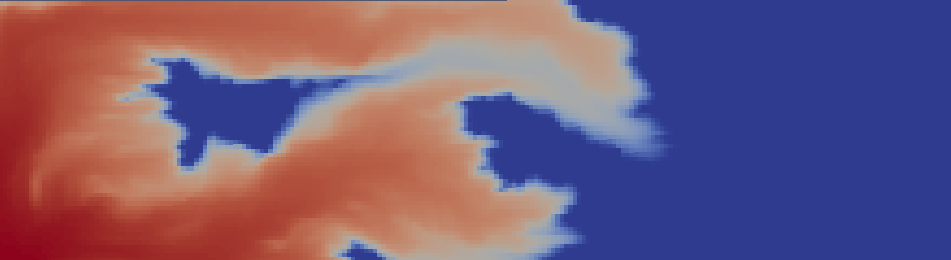
\includegraphics[width=\textwidth]{figures/saturation_tarbert_layer-0.png}
\caption{Saturation at $T = \unit[30]{d}$}
\label{fig:saturation_tarbert_layer-0}
\end{subfigure}
~
\begin{subfigure}{0.49\textwidth}
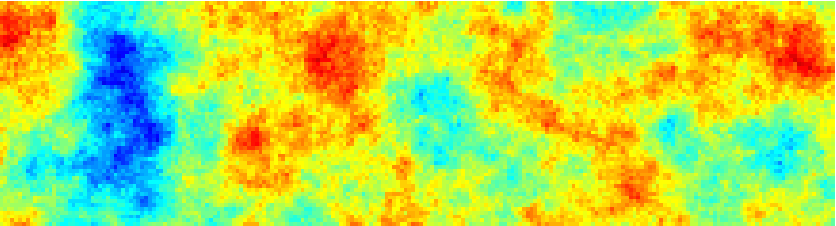
\includegraphics[width=\textwidth]{figures/perm_tarbert_layer-0.png}
\caption{Permeability}
\label{fig:perm_tarbert_layer-0}
\end{subfigure}
\caption{}
\label{fig:tarbert_layer-0}
\end{figure}

Figure \ref{fig:spe10_iterations_perm_i_0_0_0_i_50} shows the total iteration count used when solving case B using the different root finders and for varying $M$. As noted, the iteration count is orders of magnitude larger than for case A with a range from around $9\times 10^4$ up to around $1.5\times 10^7$ iterations. Again the lowest iteration count is obtained by the trust region schemes, with an advantage to the precise trust region method. The other methods also follow the pattern observed in case A, with the Brent method using the most iterations, and the regula falsi and Ridders methods slightly lower. We note that for $\Delta t \lessapprox \unit[30]{d}$ the regula falsi method has a slight advantage, while the Ridders method is better for larger time steps. 

The total CPU time is shown in Figure \ref{fig:spe10_cputime_perm_i_0_0_0_i_50}, still as a function of $\Delta t$ and for all root finders and varying $M$. Despite the quite significant differences in total iteration count spent by the root finders, as shown in Figure \ref{fig:spe10_iterations_perm_i_0_0_0_i_50}, we observe very little difference in the total CPU time spent. With $M = 0.1$ the precise trust region method and the regula falsi method are slightly better than the rest, while Ridders method is a little faster with $M = 1$. For $M = 10$ the differences are very small indeed, with the precise trust region method showing the best performance. Despite the significant iteration differences we must conclude that the solver choice is of minor importance on this test case. We hypothesize that the reason for the CPU time invariance under pressure solver choice is that the time spent by the pressure solver dominates the total run time. If this hypothesis holds the most likely explanation is that the pressure solver scales badly with cell count, since this is the most significant change in the problem setup, going from $400$ cells in case A to a total of $13200$ in the present case. The choice of pressure solver is independent of the transport solver, as discussed in Section \ref{section:seq_splitting_method}, so a more efficient pressure solver could be chosen. Thus we still want to investigate the efficiency of the transport solver under the influence of different root finders. The plots in Figure \ref{fig:spe10_cputimetrans_perm_i_0_0_0_i_50} show timing results for just the transport step in the sequential splitting method.

\begin{figure}[!ht]
\tikzsetnextfilename{spe10_iterations_perm_i_0_0_0_m_1_10_i_50_dt_1to30}
\begin{subfigure}[b]{0.49\textwidth} %%%%%%%%%%% M = 0.1 %%%%%%%%%%%%%%
\begin{tikzpicture}
    \pgfplotstablegetrowsof{datafiles/spe10-iterations-s-r-T-400-m-1-10-dim-10-10-60-220-perm-i-0-0-0-i-50.data}
    \pgfmathsetmacro\yfin{\pgfmathresult}
    \pgfmathsetmacro\yini{5}
    \begin{semilogyaxis}[
            width=0.97\textwidth,
            height=0.26\textheight,
            ymin=300000,
            ymax=15600000,
            xlabel={dt~[d]},
            ylabel={\#iterations},
            grid=both,
            skip coords between index={\yini}{\yfin}
            ]
        \addplot table[col sep=comma, trim cells=true,x=dt, y=iterations] {datafiles/spe10-iterations-s-r-T-400-m-1-10-dim-10-10-60-220-perm-i-0-0-0-i-50.data};
        \addplot table[col sep=comma, trim cells=true,x=dt, y=iterations] {datafiles/spe10-iterations-s-t-T-400-m-1-10-dim-10-10-60-220-perm-i-0-0-0-i-50.data};
        \addplot table[col sep=comma, trim cells=true,x=dt, y=iterations] {datafiles/spe10-iterations-s-a-T-400-m-1-10-dim-10-10-60-220-perm-i-0-0-0-i-50.data};
        \addplot table[col sep=comma, trim cells=true,x=dt, y=iterations] {datafiles/spe10-iterations-s-b-T-400-m-1-10-dim-10-10-60-220-perm-i-0-0-0-i-50.data};
        \addplot table[col sep=comma, trim cells=true,x=dt, y=iterations] {datafiles/spe10-iterations-s-i-T-400-m-1-10-dim-10-10-60-220-perm-i-0-0-0-i-50.data};
        \legend{RF,TR,TR*,B,R}
    \end{semilogyaxis}
\end{tikzpicture}%
\caption{$M =0.1$} \label{fig:spe10_iterations_perm_i_0_0_0_m_1_10_i_50_dt_1to30}
\end{subfigure}%
~
\tikzsetnextfilename{spe10_iterations_perm_i_0_0_0_m_1_10_i_50_dt_40to150}
\begin{subfigure}[b]{0.49\textwidth}
\begin{tikzpicture}
    \pgfplotstablegetrowsof{datafiles/spe10-iterations-s-r-T-400-m-1-10-dim-10-10-60-220-perm-i-0-0-0-i-50.data}
    \pgfmathsetmacro\yfin{5}
    \pgfmathsetmacro\yini{0}
    \begin{semilogyaxis}[
            width=0.97\textwidth,
            height=0.26\textheight,
            ymin=90000,
            ymax=1000000,
            xlabel={dt~[d]},
            ylabel={\#iterations},
            grid=both,
            skip coords between index={\yini}{\yfin}
            ]
        \addplot table[col sep=comma, trim cells=true,x=dt, y=iterations] {datafiles/spe10-iterations-s-r-T-400-m-1-10-dim-10-10-60-220-perm-i-0-0-0-i-50.data};
        \addplot table[col sep=comma, trim cells=true,x=dt, y=iterations] {datafiles/spe10-iterations-s-t-T-400-m-1-10-dim-10-10-60-220-perm-i-0-0-0-i-50.data};
        \addplot table[col sep=comma, trim cells=true,x=dt, y=iterations] {datafiles/spe10-iterations-s-a-T-400-m-1-10-dim-10-10-60-220-perm-i-0-0-0-i-50.data};
        \addplot table[col sep=comma, trim cells=true,x=dt, y=iterations] {datafiles/spe10-iterations-s-b-T-400-m-1-10-dim-10-10-60-220-perm-i-0-0-0-i-50.data};
        \addplot table[col sep=comma, trim cells=true,x=dt, y=iterations] {datafiles/spe10-iterations-s-i-T-400-m-1-10-dim-10-10-60-220-perm-i-0-0-0-i-50.data};
        %\legend{RF,TR,TR*,B,R}
    \end{semilogyaxis}
\end{tikzpicture}%
\caption{$M =0.1$} \label{fig:spe10_iterations_perm_i_0_0_0_m_1_10_i_50_dt_40to150}
\end{subfigure}%
\vspace{0.3cm} %%%%%%%%%%% M = 1 %%%%%%%%%%%%%%
\tikzsetnextfilename{spe10_iterations_perm_i_0_0_0_m_1_1_i_50_dt_1to30}
\begin{subfigure}[b]{0.49\textwidth}
\begin{tikzpicture}
    \pgfplotstablegetrowsof{datafiles/spe10-iterations-s-r-T-400-m-1-10-dim-10-10-60-220-perm-i-0-0-0-i-50.data}
    \pgfmathsetmacro\yfin{\pgfmathresult}
    \pgfmathsetmacro\yini{5}
    \begin{semilogyaxis}[
            width=0.97\textwidth,
            height=0.26\textheight,
            ymin=190000,
            ymax=11500000,
            xlabel={dt~[d]},
            ylabel={\#iterations},
            grid=both,
            skip coords between index={\yini}{\yfin}
            ]
         \addplot table[col sep=comma, trim cells=true,x=dt, y=iterations] {datafiles/spe10-iterations-s-r-T-400-m-1-1-dim-10-10-60-220-perm-i-0-0-0-i-50.data};
        \addplot table[col sep=comma, trim cells=true,x=dt, y=iterations] {datafiles/spe10-iterations-s-t-T-400-m-1-1-dim-10-10-60-220-perm-i-0-0-0-i-50.data};
        \addplot table[col sep=comma, trim cells=true,x=dt, y=iterations] {datafiles/spe10-iterations-s-a-T-400-m-1-1-dim-10-10-60-220-perm-i-0-0-0-i-50.data};
        \addplot table[col sep=comma, trim cells=true,x=dt, y=iterations] {datafiles/spe10-iterations-s-b-T-400-m-1-1-dim-10-10-60-220-perm-i-0-0-0-i-50.data};
        \addplot table[col sep=comma, trim cells=true,x=dt, y=iterations] {datafiles/spe10-iterations-s-i-T-400-m-1-1-dim-10-10-60-220-perm-i-0-0-0-i-50.data};
        \legend{RF,TR,TR*,B,R}
    \end{semilogyaxis}
\end{tikzpicture}%
\caption{$M =1$} \label{fig:spe10_iterations_perm_i_0_0_0_m_1_1_i_50_dt_1to30}
\end{subfigure}%
~
\tikzsetnextfilename{spe10_iterations_perm_i_0_0_0_m_1_1_i_50_dt_40to150}
\begin{subfigure}[b]{0.49\textwidth}
\begin{tikzpicture}
    \pgfplotstablegetrowsof{datafiles/spe10-iterations-s-r-T-400-m-1-10-dim-10-10-60-220-perm-i-0-0-0-i-50.data}
    \pgfmathsetmacro\yfin{5}
    \pgfmathsetmacro\yini{0}
    \begin{semilogyaxis}[
            width=0.97\textwidth,
            height=0.26\textheight,
            ymin=86000,
            ymax=1000000,
            xlabel={dt~[d]},
            ylabel={\#iterations},
            grid=both,
            skip coords between index={\yini}{\yfin}
            ]
         \addplot table[col sep=comma, trim cells=true,x=dt, y=iterations] {datafiles/spe10-iterations-s-r-T-400-m-1-1-dim-10-10-60-220-perm-i-0-0-0-i-50.data};
        \addplot table[col sep=comma, trim cells=true,x=dt, y=iterations] {datafiles/spe10-iterations-s-t-T-400-m-1-1-dim-10-10-60-220-perm-i-0-0-0-i-50.data};
        \addplot table[col sep=comma, trim cells=true,x=dt, y=iterations] {datafiles/spe10-iterations-s-a-T-400-m-1-1-dim-10-10-60-220-perm-i-0-0-0-i-50.data};
        \addplot table[col sep=comma, trim cells=true,x=dt, y=iterations] {datafiles/spe10-iterations-s-b-T-400-m-1-1-dim-10-10-60-220-perm-i-0-0-0-i-50.data};
        \addplot table[col sep=comma, trim cells=true,x=dt, y=iterations] {datafiles/spe10-iterations-s-i-T-400-m-1-1-dim-10-10-60-220-perm-i-0-0-0-i-50.data};
        %\legend{RF,TR,TR*,B,R}
    \end{semilogyaxis}
\end{tikzpicture}%
\caption{$M =1$} \label{fig:spe10_iterations_perm_i_0_0_0_m_1_1_i_50_dt_40to150}
\end{subfigure}%
\vspace{0.3cm} %%%%%%%%%%% M = 10 %%%%%%%%%%%%%%
\tikzsetnextfilename{spe10_iterations_perm_i_0_0_0_m_10_1_i_50_dt_1to30}
\begin{subfigure}[b]{0.49\textwidth}
\begin{tikzpicture}
    \pgfplotstablegetrowsof{datafiles/spe10-iterations-s-r-T-400-m-1-10-dim-10-10-60-220-perm-i-0-0-0-i-50.data}
    \pgfmathsetmacro\yfin{\pgfmathresult}
    \pgfmathsetmacro\yini{5}
    \begin{semilogyaxis}[
            width=0.97\textwidth,
            height=0.26\textheight,
            ymin=200000,
            ymax=10000000,
            xlabel={dt~[d]},
            ylabel={\#iterations},
            grid=both,
            skip coords between index={\yini}{\yfin}
            ]
         \addplot table[col sep=comma, trim cells=true,x=dt, y=iterations] {datafiles/spe10-iterations-s-r-T-400-m-10-1-dim-10-10-60-220-perm-i-0-0-0-i-50.data};
        \addplot table[col sep=comma, trim cells=true,x=dt, y=iterations] {datafiles/spe10-iterations-s-t-T-400-m-10-1-dim-10-10-60-220-perm-i-0-0-0-i-50.data};
        \addplot table[col sep=comma, trim cells=true,x=dt, y=iterations] {datafiles/spe10-iterations-s-a-T-400-m-10-1-dim-10-10-60-220-perm-i-0-0-0-i-50.data};
        \addplot table[col sep=comma, trim cells=true,x=dt, y=iterations] {datafiles/spe10-iterations-s-b-T-400-m-10-1-dim-10-10-60-220-perm-i-0-0-0-i-50.data};
        \addplot table[col sep=comma, trim cells=true,x=dt, y=iterations] {datafiles/spe10-iterations-s-i-T-400-m-10-1-dim-10-10-60-220-perm-i-0-0-0-i-50.data};
        \legend{RF,TR,TR*,B,R}
    \end{semilogyaxis}
\end{tikzpicture}%
\caption{$M =10$} \label{fig:spe10_iterations_perm_i_0_0_0_m_10_1_i_50_dt_1to30}
\end{subfigure}%
~
\tikzsetnextfilename{spe10_iterations_perm_i_0_0_0_m_10_1_i_50_dt_40to150}
\begin{subfigure}[b]{0.49\textwidth}
\begin{tikzpicture}
    \pgfplotstablegetrowsof{datafiles/spe10-iterations-s-r-T-400-m-1-10-dim-10-10-60-220-perm-i-0-0-0-i-50.data}
    \pgfmathsetmacro\yfin{5}
    \pgfmathsetmacro\yini{0}
    \begin{semilogyaxis}[
            width=0.97\textwidth,
            height=0.26\textheight,
            ymin=64000,
            ymax=1000000,
            xlabel={dt~[d]},
            ylabel={\#iterations},
            grid=both,
            skip coords between index={\yini}{\yfin}
            ]
         \addplot table[col sep=comma, trim cells=true,x=dt, y=iterations] {datafiles/spe10-iterations-s-r-T-400-m-10-1-dim-10-10-60-220-perm-i-0-0-0-i-50.data};
        \addplot table[col sep=comma, trim cells=true,x=dt, y=iterations] {datafiles/spe10-iterations-s-t-T-400-m-10-1-dim-10-10-60-220-perm-i-0-0-0-i-50.data};
        \addplot table[col sep=comma, trim cells=true,x=dt, y=iterations] {datafiles/spe10-iterations-s-a-T-400-m-10-1-dim-10-10-60-220-perm-i-0-0-0-i-50.data};
        \addplot table[col sep=comma, trim cells=true,x=dt, y=iterations] {datafiles/spe10-iterations-s-b-T-400-m-10-1-dim-10-10-60-220-perm-i-0-0-0-i-50.data};
        \addplot table[col sep=comma, trim cells=true,x=dt, y=iterations] {datafiles/spe10-iterations-s-i-T-400-m-10-1-dim-10-10-60-220-perm-i-0-0-0-i-50.data};
        %\legend{RF,TR,TR*,B,R}
    \end{semilogyaxis}
\end{tikzpicture}%
\caption{$M =10$} \label{fig:spe10_iterations_perm_i_0_0_0_m_10_1_i_50_dt_40to150}
\end{subfigure}%
\caption{\#iterations used to solve case B, Section \ref{section:caseB}, for varying root finders, time steps and viscosity ratios.}
\label{fig:spe10_iterations_perm_i_0_0_0_i_50}
\end{figure}%
%
%\begin{figure}[!ht]
%\centering
%\tikzsetnextfilename{spe10_iterations_perm_i_0_0_0_m_1_10_i_50}
%\begin{subfigure}[b]{0.8\textwidth}
%\begin{tikzpicture}
%    \pgfplotstablegetrowsof{datafiles/spe10-iterations-s-r-T-400-m-1-10-dim-10-10-60-220-perm-i-0-0-0-i-50.data}
%    \pgfmathsetmacro\yfin{\pgfmathresult - 4}
%    \pgfmathsetmacro\yini{0}
%    \begin{semilogyaxis}[
%            width=0.97\textwidth,
%            height=0.26\textheight,
%            ymin=40000,
%            ymax=30000000,
%            xlabel={dt~[d]},
%            ylabel={\#iterations},
%            grid=both,
%            ]
%        \addplot table[col sep=comma, trim cells=true,x=dt, y=iterations] {datafiles/spe10-iterations-s-r-T-400-m-1-10-dim-10-10-60-220-perm-i-0-0-0-i-50.data};
%        \addplot table[col sep=comma, trim cells=true,x=dt, y=iterations] {datafiles/spe10-iterations-s-t-T-400-m-1-10-dim-10-10-60-220-perm-i-0-0-0-i-50.data};
%        \addplot table[col sep=comma, trim cells=true,x=dt, y=iterations] {datafiles/spe10-iterations-s-a-T-400-m-1-10-dim-10-10-60-220-perm-i-0-0-0-i-50.data};
%        \addplot table[col sep=comma, trim cells=true,x=dt, y=iterations] {datafiles/spe10-iterations-s-b-T-400-m-1-10-dim-10-10-60-220-perm-i-0-0-0-i-50.data};
%        \addplot table[col sep=comma, trim cells=true,x=dt, y=iterations] {datafiles/spe10-iterations-s-i-T-400-m-1-10-dim-10-10-60-220-perm-i-0-0-0-i-50.data};
%                %\addplot table[col sep=comma, trim cells=true,x=dt, y=iterations] {datafiles/spe10-iterations-s-g-T-400-m-1-10-dim-10-10-60-220-perm-i-0-0-0-i-50.data};
%        \legend{RF,TR,TR*,B,R}
%    \end{semilogyaxis}
%\end{tikzpicture}%
%\caption{$M =0.1$} \label{fig:spe10_iterations_perm_i_0_0_0_m_1_10_i_50}
%\end{subfigure}%
%\vspace{0.3cm}
%\centering
%\tikzsetnextfilename{spe10_iterations_perm_i_0_0_0_m_1_1_i_50}
%\begin{subfigure}[b]{0.8\textwidth}
%\begin{tikzpicture}
%    \begin{semilogyaxis}[
%            width=0.97\textwidth,
%            height=0.26\textheight,
%            ymin=40000,
%            ymax=30000000,
%            xlabel={dt~[d]},
%            ylabel={\#iterations},
%            grid=both,
%            ]
%         \addplot table[col sep=comma, trim cells=true,x=dt, y=iterations] {datafiles/spe10-iterations-s-r-T-400-m-1-1-dim-10-10-60-220-perm-i-0-0-0-i-50.data};
%        \addplot table[col sep=comma, trim cells=true,x=dt, y=iterations] {datafiles/spe10-iterations-s-t-T-400-m-1-1-dim-10-10-60-220-perm-i-0-0-0-i-50.data};
%        \addplot table[col sep=comma, trim cells=true,x=dt, y=iterations] {datafiles/spe10-iterations-s-a-T-400-m-1-1-dim-10-10-60-220-perm-i-0-0-0-i-50.data};
%        \addplot table[col sep=comma, trim cells=true,x=dt, y=iterations] {datafiles/spe10-iterations-s-b-T-400-m-1-1-dim-10-10-60-220-perm-i-0-0-0-i-50.data};
%        \addplot table[col sep=comma, trim cells=true,x=dt, y=iterations] {datafiles/spe10-iterations-s-i-T-400-m-1-1-dim-10-10-60-220-perm-i-0-0-0-i-50.data};
%                %\addplot table[col sep=comma, trim cells=true,x=dt, y=iterations] {datafiles/spe10-iterations-s-g-T-400-m-1-1-dim-10-10-60-220-perm-i-0-0-0-i-50.data};
%        \legend{RF,TR,TR*,B,R}
%    \end{semilogyaxis}
%\end{tikzpicture}%
%\caption{$M =1$} \label{fig:spe10_iterations_perm_i_0_0_0_m_1_1_i_50}
%\end{subfigure}%
%\vspace{0.3cm}
%\centering
%\tikzsetnextfilename{spe10_iterations_perm_i_0_0_0_m_10_1_i_50}
%\begin{subfigure}[b]{0.8\textwidth}
%\begin{tikzpicture}
%    \begin{semilogyaxis}[
%            width=0.97\textwidth,
%            height=0.26\textheight,
%            ymin=40000,
%            ymax=30000000,
%            xlabel={dt~[d]},
%            ylabel={\#iterations},
%            grid=both,
%            ]
%         \addplot table[col sep=comma, trim cells=true,x=dt, y=iterations] {datafiles/spe10-iterations-s-r-T-400-m-10-1-dim-10-10-60-220-perm-i-0-0-0-i-50.data};
%        \addplot table[col sep=comma, trim cells=true,x=dt, y=iterations] {datafiles/spe10-iterations-s-t-T-400-m-10-1-dim-10-10-60-220-perm-i-0-0-0-i-50.data};
%        \addplot table[col sep=comma, trim cells=true,x=dt, y=iterations] {datafiles/spe10-iterations-s-a-T-400-m-10-1-dim-10-10-60-220-perm-i-0-0-0-i-50.data};
%        \addplot table[col sep=comma, trim cells=true,x=dt, y=iterations] {datafiles/spe10-iterations-s-b-T-400-m-10-1-dim-10-10-60-220-perm-i-0-0-0-i-50.data};
%        \addplot table[col sep=comma, trim cells=true,x=dt, y=iterations] {datafiles/spe10-iterations-s-i-T-400-m-10-1-dim-10-10-60-220-perm-i-0-0-0-i-50.data};
%                %\addplot table[col sep=comma, trim cells=true,x=dt, y=iterations] {datafiles/spe10-iterations-s-g-T-400-m-10-1-dim-10-10-60-220-perm-i-0-0-0-i-50.data};
%        \legend{RF,TR,TR*,B,R}
%    \end{semilogyaxis}
%\end{tikzpicture}%
%\caption{$M =10$} \label{fig:spe10_iterations_perm_i_0_0_0_m_10_1_i_50}
%\end{subfigure}%
%\caption{\#iterations used to solve the Q5 problem, Section \ref{section:caseA}, for varying root finders, time steps and viscosity ratios.}
%\label{fig:spe10_iterations_perm_i_0_0_0_i_50}
%\end{figure}
%\begin{figure}[!ht]
\centering
\tikzsetnextfilename{spe10_cputime_perm_i_0_0_0_m_1_10_i_50}
\begin{subfigure}[b]{0.8\textwidth}
\begin{tikzpicture}
    \begin{semilogyaxis}[
            width=0.97\textwidth,
            height=0.26\textheight,
            xlabel={dt~[d]},
            ylabel={CPU time~[s]},
            grid=both,
            ]
        \addplot table[col sep=comma, trim cells=true,x=dt, y=cputime] {datafiles/spe10-cputvsdt-s-r-T-400-m-1-10-dim-10-10-60-220-perm-i-0-0-0-i-50.data};
        \addplot table[col sep=comma, trim cells=true,x=dt, y=cputime] {datafiles/spe10-cputvsdt-s-t-T-400-m-1-10-dim-10-10-60-220-perm-i-0-0-0-i-50.data};
        \addplot table[col sep=comma, trim cells=true,x=dt, y=cputime] {datafiles/spe10-cputvsdt-s-a-T-400-m-1-10-dim-10-10-60-220-perm-i-0-0-0-i-50.data};
        \addplot table[col sep=comma, trim cells=true,x=dt, y=cputime] {datafiles/spe10-cputvsdt-s-b-T-400-m-1-10-dim-10-10-60-220-perm-i-0-0-0-i-50.data};
        \addplot table[col sep=comma, trim cells=true,x=dt, y=cputime] {datafiles/spe10-cputvsdt-s-i-T-400-m-1-10-dim-10-10-60-220-perm-i-0-0-0-i-50.data};                
        \legend{RF,TR,TR*,B,R}
    \end{semilogyaxis}
\end{tikzpicture}%
\caption{$M =0.1$} \label{fig:spe10_cputime_perm_i_0_0_0_m_1_10_i_50}
\end{subfigure}%
\vspace{0.3cm}
\centering
\tikzsetnextfilename{spe10_cputime_perm_i_0_0_0_m_1_1_i_50}
\begin{subfigure}[b]{0.8\textwidth}
\begin{tikzpicture}
    \begin{semilogyaxis}[
            width=0.97\textwidth,
            height=0.26\textheight,
            xlabel={dt~[d]},
            ylabel={CPU time~[s]},
            grid=both,
            ]
         \addplot table[col sep=comma, trim cells=true,x=dt, y=cputime] {datafiles/spe10-cputvsdt-s-r-T-400-m-1-1-dim-10-10-60-220-perm-i-0-0-0-i-50.data};
        \addplot table[col sep=comma, trim cells=true,x=dt, y=cputime] {datafiles/spe10-cputvsdt-s-t-T-400-m-1-1-dim-10-10-60-220-perm-i-0-0-0-i-50.data};
        \addplot table[col sep=comma, trim cells=true,x=dt, y=cputime] {datafiles/spe10-cputvsdt-s-a-T-400-m-1-1-dim-10-10-60-220-perm-i-0-0-0-i-50.data};
        \addplot table[col sep=comma, trim cells=true,x=dt, y=cputime] {datafiles/spe10-cputvsdt-s-b-T-400-m-1-1-dim-10-10-60-220-perm-i-0-0-0-i-50.data};
        \addplot table[col sep=comma, trim cells=true,x=dt, y=cputime] {datafiles/spe10-cputvsdt-s-i-T-400-m-1-1-dim-10-10-60-220-perm-i-0-0-0-i-50.data};
        \legend{RF,TR,TR*,B,R}
    \end{semilogyaxis}
\end{tikzpicture}%
\caption{$M =1$} \label{fig:spe10_cputime_perm_i_0_0_0_m_1_1_i_50}
\end{subfigure}%
\vspace{0.3cm}
\centering
\tikzsetnextfilename{spe10_cputime_perm_i_0_0_0_m_10_1_i_50}
\begin{subfigure}[b]{0.8\textwidth}
\begin{tikzpicture}
    \begin{semilogyaxis}[
            width=0.97\textwidth,
            height=0.26\textheight,
            xlabel={dt~[d]},
            ylabel={CPU time~[s]},
            grid=both,
            ]
         \addplot table[col sep=comma, trim cells=true,x=dt, y=cputime] {datafiles/spe10-cputvsdt-s-r-T-400-m-10-1-dim-10-10-60-220-perm-i-0-0-0-i-50.data};
        \addplot table[col sep=comma, trim cells=true,x=dt, y=cputime] {datafiles/spe10-cputvsdt-s-t-T-400-m-10-1-dim-10-10-60-220-perm-i-0-0-0-i-50.data};
        \addplot table[col sep=comma, trim cells=true,x=dt, y=cputime] {datafiles/spe10-cputvsdt-s-a-T-400-m-10-1-dim-10-10-60-220-perm-i-0-0-0-i-50.data};
        \addplot table[col sep=comma, trim cells=true,x=dt, y=cputime] {datafiles/spe10-cputvsdt-s-b-T-400-m-10-1-dim-10-10-60-220-perm-i-0-0-0-i-50.data};
        \addplot table[col sep=comma, trim cells=true,x=dt, y=cputime] {datafiles/spe10-cputvsdt-s-i-T-400-m-10-1-dim-10-10-60-220-perm-i-0-0-0-i-50.data};
        \legend{RF,TR,TR*,B,R}
    \end{semilogyaxis}
\end{tikzpicture}%
\caption{$M =10$} \label{fig:spe10_cputime_perm_i_0_0_0_m_10_1_i_50}
\end{subfigure}%
\caption{CPU time used to solve case B, Section \ref{section:caseB}, for varying root finders, time steps and viscosity ratios.}
\label{fig:spe10_cputime_perm_i_0_0_0_i_50}
\end{figure}
\begin{figure}[!ht]
\tikzsetnextfilename{spe10_cputime_perm_i_0_0_0_m_1_10_i_50_dt_1to30}
\begin{subfigure}[b]{0.49\textwidth} %%%%%%%%%%% M = 0.1 %%%%%%%%%%%%%%
\centering
\begin{tikzpicture}
    \pgfplotstablegetrowsof{datafiles/spe10-cputvsdt-s-r-T-400-m-1-10-dim-10-10-60-220-perm-i-0-0-0-i-50.data}
    \pgfmathsetmacro\yfin{\pgfmathresult}
    \pgfmathsetmacro\yini{4}
    \begin{semilogyaxis}[
            width=0.97\textwidth,
            height=0.26\textheight,
            ymin=1,
            ymax=100,
            xlabel={dt~[d]},
            ylabel={CPU time~[s]},
            grid=both,
            skip coords between index={\yini}{\yfin}
            ]
        \addplot table[col sep=comma, trim cells=true,x=dt, y=cputime] {datafiles/spe10-cputvsdt-s-r-T-400-m-1-10-dim-10-10-60-220-perm-i-0-0-0-i-50.data};
        \addplot table[col sep=comma, trim cells=true,x=dt, y=cputime] {datafiles/spe10-cputvsdt-s-t-T-400-m-1-10-dim-10-10-60-220-perm-i-0-0-0-i-50.data};
        \addplot table[col sep=comma, trim cells=true,x=dt, y=cputime] {datafiles/spe10-cputvsdt-s-a-T-400-m-1-10-dim-10-10-60-220-perm-i-0-0-0-i-50.data};
        \addplot table[col sep=comma, trim cells=true,x=dt, y=cputime] {datafiles/spe10-cputvsdt-s-b-T-400-m-1-10-dim-10-10-60-220-perm-i-0-0-0-i-50.data};
        \addplot table[col sep=comma, trim cells=true,x=dt, y=cputime] {datafiles/spe10-cputvsdt-s-i-T-400-m-1-10-dim-10-10-60-220-perm-i-0-0-0-i-50.data};
        \legend{RF,TR,TR*,B,R}
    \end{semilogyaxis}
\end{tikzpicture}%
\caption{$M =0.1$} \label{fig:spe10_cputime_perm_i_0_0_0_m_1_10_i_50_dt_1to30}
\end{subfigure}%
~
\tikzsetnextfilename{spe10_cputime_perm_i_0_0_0_m_1_10_i_50_dt_40to150}
\begin{subfigure}[b]{0.49\textwidth}
\centering
\begin{tikzpicture}
    \pgfplotstablegetrowsof{datafiles/spe10-cputvsdt-s-r-T-400-m-1-10-dim-10-10-60-220-perm-i-0-0-0-i-50.data}
    \pgfmathsetmacro\yfin{4}
    \pgfmathsetmacro\yini{0}
    \begin{semilogyaxis}[
            width=0.97\textwidth,
            height=0.26\textheight,
            ymin=0.1,
            ymax=2,
            xlabel={dt~[d]},
            ylabel={CPU time~[s]},
            grid=both,
            skip coords between index={\yini}{\yfin}
            ]
        \addplot table[col sep=comma, trim cells=true,x=dt, y=cputime] {datafiles/spe10-cputvsdt-s-r-T-400-m-1-10-dim-10-10-60-220-perm-i-0-0-0-i-50.data};
        \addplot table[col sep=comma, trim cells=true,x=dt, y=cputime] {datafiles/spe10-cputvsdt-s-t-T-400-m-1-10-dim-10-10-60-220-perm-i-0-0-0-i-50.data};
        \addplot table[col sep=comma, trim cells=true,x=dt, y=cputime] {datafiles/spe10-cputvsdt-s-a-T-400-m-1-10-dim-10-10-60-220-perm-i-0-0-0-i-50.data};
        \addplot table[col sep=comma, trim cells=true,x=dt, y=cputime] {datafiles/spe10-cputvsdt-s-b-T-400-m-1-10-dim-10-10-60-220-perm-i-0-0-0-i-50.data};
        \addplot table[col sep=comma, trim cells=true,x=dt, y=cputime] {datafiles/spe10-cputvsdt-s-i-T-400-m-1-10-dim-10-10-60-220-perm-i-0-0-0-i-50.data};
        %\legend{RF,TR,TR*,B,R}
    \end{semilogyaxis}
\end{tikzpicture}%
\caption{$M =0.1$} \label{fig:spe10_cputime_perm_i_0_0_0_m_1_10_i_50_dt_40to150}
\end{subfigure}%
\vspace{0.3cm} %%%%%%%%%%% M = 1 %%%%%%%%%%%%%%
\tikzsetnextfilename{spe10_cputime_perm_i_0_0_0_m_1_1_i_50_dt_1to30}
\begin{subfigure}[b]{0.49\textwidth}
\centering
\begin{tikzpicture}
    \pgfplotstablegetrowsof{datafiles/spe10-cputvsdt-s-r-T-400-m-1-10-dim-10-10-60-220-perm-i-0-0-0-i-50.data}
    \pgfmathsetmacro\yfin{\pgfmathresult}
    \pgfmathsetmacro\yini{4}
    \begin{semilogyaxis}[
            width=0.97\textwidth,
            height=0.26\textheight,
            ymin=1,
            ymax=100,
            xlabel={dt~[d]},
            ylabel={CPU time~[s]},
            grid=both,
            skip coords between index={\yini}{\yfin}
            ]
         \addplot table[col sep=comma, trim cells=true,x=dt, y=cputime] {datafiles/spe10-cputvsdt-s-r-T-400-m-1-1-dim-10-10-60-220-perm-i-0-0-0-i-50.data};
        \addplot table[col sep=comma, trim cells=true,x=dt, y=cputime] {datafiles/spe10-cputvsdt-s-t-T-400-m-1-1-dim-10-10-60-220-perm-i-0-0-0-i-50.data};
        \addplot table[col sep=comma, trim cells=true,x=dt, y=cputime] {datafiles/spe10-cputvsdt-s-a-T-400-m-1-1-dim-10-10-60-220-perm-i-0-0-0-i-50.data};
        \addplot table[col sep=comma, trim cells=true,x=dt, y=cputime] {datafiles/spe10-cputvsdt-s-b-T-400-m-1-1-dim-10-10-60-220-perm-i-0-0-0-i-50.data};
        \addplot table[col sep=comma, trim cells=true,x=dt, y=cputime] {datafiles/spe10-cputvsdt-s-i-T-400-m-1-1-dim-10-10-60-220-perm-i-0-0-0-i-50.data};
        \legend{RF,TR,TR*,B,R}
    \end{semilogyaxis}
\end{tikzpicture}%
\caption{$M =1$} \label{fig:spe10_cputime_perm_i_0_0_0_m_1_1_i_50_dt_1to30}
\end{subfigure}%
~
\tikzsetnextfilename{spe10_cputime_perm_i_0_0_0_m_1_1_i_50_dt_40to150}
\begin{subfigure}[b]{0.49\textwidth}
\centering
\begin{tikzpicture}
    \pgfplotstablegetrowsof{datafiles/spe10-cputvsdt-s-r-T-400-m-1-10-dim-10-10-60-220-perm-i-0-0-0-i-50.data}
    \pgfmathsetmacro\yfin{4}
    \pgfmathsetmacro\yini{0}
    \begin{semilogyaxis}[
            width=0.97\textwidth,
            height=0.26\textheight,
            ymin=0.1,
            ymax=2,
            xlabel={dt~[d]},
            ylabel={CPU time~[s]},
            grid=both,
            skip coords between index={\yini}{\yfin}
            ]
         \addplot table[col sep=comma, trim cells=true,x=dt, y=cputime] {datafiles/spe10-cputvsdt-s-r-T-400-m-1-1-dim-10-10-60-220-perm-i-0-0-0-i-50.data};
        \addplot table[col sep=comma, trim cells=true,x=dt, y=cputime] {datafiles/spe10-cputvsdt-s-t-T-400-m-1-1-dim-10-10-60-220-perm-i-0-0-0-i-50.data};
        \addplot table[col sep=comma, trim cells=true,x=dt, y=cputime] {datafiles/spe10-cputvsdt-s-a-T-400-m-1-1-dim-10-10-60-220-perm-i-0-0-0-i-50.data};
        \addplot table[col sep=comma, trim cells=true,x=dt, y=cputime] {datafiles/spe10-cputvsdt-s-b-T-400-m-1-1-dim-10-10-60-220-perm-i-0-0-0-i-50.data};
        \addplot table[col sep=comma, trim cells=true,x=dt, y=cputime] {datafiles/spe10-cputvsdt-s-i-T-400-m-1-1-dim-10-10-60-220-perm-i-0-0-0-i-50.data};
        %\legend{RF,TR,TR*,B,R}
    \end{semilogyaxis}
\end{tikzpicture}%
\caption{$M =1$} \label{fig:spe10_cputime_perm_i_0_0_0_m_1_1_i_50_dt_40to150}
\end{subfigure}%
\vspace{0.3cm} %%%%%%%%%%% M = 10 %%%%%%%%%%%%%%
\tikzsetnextfilename{spe10_cputime_perm_i_0_0_0_m_10_1_i_50_dt_1to30}
\begin{subfigure}[b]{0.49\textwidth}
\centering
\begin{tikzpicture}
    \pgfplotstablegetrowsof{datafiles/spe10-cputvsdt-s-r-T-400-m-1-10-dim-10-10-60-220-perm-i-0-0-0-i-50.data}
    \pgfmathsetmacro\yfin{\pgfmathresult}
    \pgfmathsetmacro\yini{4}
    \begin{semilogyaxis}[
            width=0.97\textwidth,
            height=0.26\textheight,
            ymin=1,
            ymax=100,
            xlabel={dt~[d]},
            ylabel={CPU time~[s]},
            grid=both,
            skip coords between index={\yini}{\yfin}
            ]
         \addplot table[col sep=comma, trim cells=true,x=dt, y=cputime] {datafiles/spe10-cputvsdt-s-r-T-400-m-10-1-dim-10-10-60-220-perm-i-0-0-0-i-50.data};
        \addplot table[col sep=comma, trim cells=true,x=dt, y=cputime] {datafiles/spe10-cputvsdt-s-t-T-400-m-10-1-dim-10-10-60-220-perm-i-0-0-0-i-50.data};
        \addplot table[col sep=comma, trim cells=true,x=dt, y=cputime] {datafiles/spe10-cputvsdt-s-a-T-400-m-10-1-dim-10-10-60-220-perm-i-0-0-0-i-50.data};
        \addplot table[col sep=comma, trim cells=true,x=dt, y=cputime] {datafiles/spe10-cputvsdt-s-b-T-400-m-10-1-dim-10-10-60-220-perm-i-0-0-0-i-50.data};
        \addplot table[col sep=comma, trim cells=true,x=dt, y=cputime] {datafiles/spe10-cputvsdt-s-i-T-400-m-10-1-dim-10-10-60-220-perm-i-0-0-0-i-50.data};
        \legend{RF,TR,TR*,B,R}
    \end{semilogyaxis}
\end{tikzpicture}%
\caption{$M =10$} \label{fig:spe10_cputime_perm_i_0_0_0_m_10_1_i_50_dt_1to30}
\end{subfigure}%
~
\tikzsetnextfilename{spe10_cputime_perm_i_0_0_0_m_10_1_i_50_dt_40to150}
\begin{subfigure}[b]{0.49\textwidth}
\centering
\begin{tikzpicture}
    \pgfplotstablegetrowsof{datafiles/spe10-cputvsdt-s-r-T-400-m-1-10-dim-10-10-60-220-perm-i-0-0-0-i-50.data}
    \pgfmathsetmacro\yfin{4}
    \pgfmathsetmacro\yini{0}
    \begin{semilogyaxis}[
            width=0.97\textwidth,
            height=0.26\textheight,
            ymin=0.1,
            ymax=2,
            xlabel={dt~[d]},
            ylabel={CPU time~[s]},
            grid=both,
            skip coords between index={\yini}{\yfin}
            ]
         \addplot table[col sep=comma, trim cells=true,x=dt, y=cputime] {datafiles/spe10-cputvsdt-s-r-T-400-m-10-1-dim-10-10-60-220-perm-i-0-0-0-i-50.data};
        \addplot table[col sep=comma, trim cells=true,x=dt, y=cputime] {datafiles/spe10-cputvsdt-s-t-T-400-m-10-1-dim-10-10-60-220-perm-i-0-0-0-i-50.data};
        \addplot table[col sep=comma, trim cells=true,x=dt, y=cputime] {datafiles/spe10-cputvsdt-s-a-T-400-m-10-1-dim-10-10-60-220-perm-i-0-0-0-i-50.data};
        \addplot table[col sep=comma, trim cells=true,x=dt, y=cputime] {datafiles/spe10-cputvsdt-s-b-T-400-m-10-1-dim-10-10-60-220-perm-i-0-0-0-i-50.data};
        \addplot table[col sep=comma, trim cells=true,x=dt, y=cputime] {datafiles/spe10-cputvsdt-s-i-T-400-m-10-1-dim-10-10-60-220-perm-i-0-0-0-i-50.data};
        %\legend{RF,TR,TR*,B,R}
    \end{semilogyaxis}
\end{tikzpicture}%
\caption{$M =10$} \label{fig:spe10_cputime_perm_i_0_0_0_m_10_1_i_50_dt_40to150}
\end{subfigure}%
\caption{CPU time used to solve case B, Section \ref{section:caseB}, for varying root finders, time steps and viscosity ratios.}
\label{fig:spe10_cputime_perm_i_0_0_0_i_50}
\end{figure}%
%
%\begin{figure}[!ht]
%\centering
%\tikzsetnextfilename{spe10_cputime_perm_i_0_0_0_m_1_10_i_50}
%\begin{subfigure}[b]{0.8\textwidth}
%\begin{tikzpicture}
%    \pgfplotstablegetrowsof{datafiles/spe10-cputvsdt-s-r-T-400-m-1-10-dim-10-10-60-220-perm-i-0-0-0-i-50.data}
%    \pgfmathsetmacro\yfin{\pgfmathresult - 4}
%    \pgfmathsetmacro\yini{0}
%    \begin{semilogyaxis}[
%            width=0.97\textwidth,
%            height=0.26\textheight,
%            ymin=40000,
%            ymax=30000000,
%            xlabel={dt~[d]},
%            ylabel={CPU time~[s]},
%            grid=both,
%            ]
%        \addplot table[col sep=comma, trim cells=true,x=dt, y=cputime] {datafiles/spe10-cputvsdt-s-r-T-400-m-1-10-dim-10-10-60-220-perm-i-0-0-0-i-50.data};
%        \addplot table[col sep=comma, trim cells=true,x=dt, y=cputime] {datafiles/spe10-cputvsdt-s-t-T-400-m-1-10-dim-10-10-60-220-perm-i-0-0-0-i-50.data};
%        \addplot table[col sep=comma, trim cells=true,x=dt, y=cputime] {datafiles/spe10-cputvsdt-s-a-T-400-m-1-10-dim-10-10-60-220-perm-i-0-0-0-i-50.data};
%        \addplot table[col sep=comma, trim cells=true,x=dt, y=cputime] {datafiles/spe10-cputvsdt-s-b-T-400-m-1-10-dim-10-10-60-220-perm-i-0-0-0-i-50.data};
%        \addplot table[col sep=comma, trim cells=true,x=dt, y=cputime] {datafiles/spe10-cputvsdt-s-i-T-400-m-1-10-dim-10-10-60-220-perm-i-0-0-0-i-50.data};
%                %\addplot table[col sep=comma, trim cells=true,x=dt, y=cputime] {datafiles/spe10-cputvsdt-s-g-T-400-m-1-10-dim-10-10-60-220-perm-i-0-0-0-i-50.data};
%        \legend{RF,TR,TR*,B,R}
%    \end{semilogyaxis}
%\end{tikzpicture}%
%\caption{$M =0.1$} \label{fig:spe10_cputime_perm_i_0_0_0_m_1_10_i_50}
%\end{subfigure}%
%\vspace{0.3cm}
%\centering
%\tikzsetnextfilename{spe10_cputime_perm_i_0_0_0_m_1_1_i_50}
%\begin{subfigure}[b]{0.8\textwidth}
%\begin{tikzpicture}
%    \begin{semilogyaxis}[
%            width=0.97\textwidth,
%            height=0.26\textheight,
%            ymin=40000,
%            ymax=30000000,
%            xlabel={dt~[d]},
%            ylabel={CPU time~[s]},
%            grid=both,
%            ]
%         \addplot table[col sep=comma, trim cells=true,x=dt, y=cputime] {datafiles/spe10-cputvsdt-s-r-T-400-m-1-1-dim-10-10-60-220-perm-i-0-0-0-i-50.data};
%        \addplot table[col sep=comma, trim cells=true,x=dt, y=cputime] {datafiles/spe10-cputvsdt-s-t-T-400-m-1-1-dim-10-10-60-220-perm-i-0-0-0-i-50.data};
%        \addplot table[col sep=comma, trim cells=true,x=dt, y=cputime] {datafiles/spe10-cputvsdt-s-a-T-400-m-1-1-dim-10-10-60-220-perm-i-0-0-0-i-50.data};
%        \addplot table[col sep=comma, trim cells=true,x=dt, y=cputime] {datafiles/spe10-cputvsdt-s-b-T-400-m-1-1-dim-10-10-60-220-perm-i-0-0-0-i-50.data};
%        \addplot table[col sep=comma, trim cells=true,x=dt, y=cputime] {datafiles/spe10-cputvsdt-s-i-T-400-m-1-1-dim-10-10-60-220-perm-i-0-0-0-i-50.data};
%                %\addplot table[col sep=comma, trim cells=true,x=dt, y=cputime] {datafiles/spe10-cputvsdt-s-g-T-400-m-1-1-dim-10-10-60-220-perm-i-0-0-0-i-50.data};
%        \legend{RF,TR,TR*,B,R}
%    \end{semilogyaxis}
%\end{tikzpicture}%
%\caption{$M =1$} \label{fig:spe10_cputime_perm_i_0_0_0_m_1_1_i_50}
%\end{subfigure}%
%\vspace{0.3cm}
%\centering
%\tikzsetnextfilename{spe10_cputime_perm_i_0_0_0_m_10_1_i_50}
%\begin{subfigure}[b]{0.8\textwidth}
%\begin{tikzpicture}
%    \begin{semilogyaxis}[
%            width=0.97\textwidth,
%            height=0.26\textheight,
%            ymin=40000,
%            ymax=30000000,
%            xlabel={dt~[d]},
%            ylabel={CPU time~[s]},
%            grid=both,
%            ]
%         \addplot table[col sep=comma, trim cells=true,x=dt, y=cputime] {datafiles/spe10-cputvsdt-s-r-T-400-m-10-1-dim-10-10-60-220-perm-i-0-0-0-i-50.data};
%        \addplot table[col sep=comma, trim cells=true,x=dt, y=cputime] {datafiles/spe10-cputvsdt-s-t-T-400-m-10-1-dim-10-10-60-220-perm-i-0-0-0-i-50.data};
%        \addplot table[col sep=comma, trim cells=true,x=dt, y=cputime] {datafiles/spe10-cputvsdt-s-a-T-400-m-10-1-dim-10-10-60-220-perm-i-0-0-0-i-50.data};
%        \addplot table[col sep=comma, trim cells=true,x=dt, y=cputime] {datafiles/spe10-cputvsdt-s-b-T-400-m-10-1-dim-10-10-60-220-perm-i-0-0-0-i-50.data};
%        \addplot table[col sep=comma, trim cells=true,x=dt, y=cputime] {datafiles/spe10-cputvsdt-s-i-T-400-m-10-1-dim-10-10-60-220-perm-i-0-0-0-i-50.data};
%                %\addplot table[col sep=comma, trim cells=true,x=dt, y=cputime] {datafiles/spe10-cputvsdt-s-g-T-400-m-10-1-dim-10-10-60-220-perm-i-0-0-0-i-50.data};
%        \legend{RF,TR,TR*,B,R}
%    \end{semilogyaxis}
%\end{tikzpicture}%
%\caption{$M =10$} \label{fig:spe10_cputime_perm_i_0_0_0_m_10_1_i_50}
%\end{subfigure}%
%\caption{CPU time~[s] used to solve the Q5 problem, Section \ref{section:caseA}, for varying root finders, time steps and viscosity ratios.}
%\label{fig:spe10_cputime_perm_i_0_0_0_i_50}
%\end{figure}

\begin{figure}[!ht]
\centering
\tikzsetnextfilename{spe10_cputimetrans_perm_i_0_0_0_m_1_10_i_50}
\begin{subfigure}[b]{0.8\textwidth}
\begin{tikzpicture}
    \begin{semilogyaxis}[
            width=0.97\textwidth,
            height=0.26\textheight,
            xlabel={dt~[d]},
            ylabel={CPU time~[s]},
            grid=both,
            ]
        \addplot table[col sep=comma, trim cells=true,x=dt, y=cputime] {datafiles/spe10-cputransvsdt-s-r-T-400-m-1-10-dim-10-10-60-220-perm-i-0-0-0-i-50.data};
        \addplot table[col sep=comma, trim cells=true,x=dt, y=cputime] {datafiles/spe10-cputransvsdt-s-t-T-400-m-1-10-dim-10-10-60-220-perm-i-0-0-0-i-50.data};
        \addplot table[col sep=comma, trim cells=true,x=dt, y=cputime] {datafiles/spe10-cputransvsdt-s-a-T-400-m-1-10-dim-10-10-60-220-perm-i-0-0-0-i-50.data};
        \addplot table[col sep=comma, trim cells=true,x=dt, y=cputime] {datafiles/spe10-cputransvsdt-s-b-T-400-m-1-10-dim-10-10-60-220-perm-i-0-0-0-i-50.data};
        \addplot table[col sep=comma, trim cells=true,x=dt, y=cputime] {datafiles/spe10-cputransvsdt-s-i-T-400-m-1-10-dim-10-10-60-220-perm-i-0-0-0-i-50.data};                
        \legend{RF,TR,TR*,B,R}
    \end{semilogyaxis}
\end{tikzpicture}%
\caption{$M =0.1$} \label{fig:spe10_cputimetrans_perm_i_0_0_0_m_1_10_i_50}
\end{subfigure}%
\vspace{0.3cm}
\centering
\tikzsetnextfilename{spe10_cputimetrans_perm_i_0_0_0_m_1_1_i_50}	
\begin{subfigure}[b]{0.8\textwidth}
\begin{tikzpicture}
    \begin{semilogyaxis}[
            width=0.97\textwidth,
            height=0.26\textheight,
            xlabel={dt~[d]},
            ylabel={CPU time~[s]},
            grid=both,
            ]
         \addplot table[col sep=comma, trim cells=true,x=dt, y=cputime] {datafiles/spe10-cputransvsdt-s-r-T-400-m-1-1-dim-10-10-60-220-perm-i-0-0-0-i-50.data};
        \addplot table[col sep=comma, trim cells=true,x=dt, y=cputime] {datafiles/spe10-cputransvsdt-s-t-T-400-m-1-1-dim-10-10-60-220-perm-i-0-0-0-i-50.data};
        \addplot table[col sep=comma, trim cells=true,x=dt, y=cputime] {datafiles/spe10-cputransvsdt-s-a-T-400-m-1-1-dim-10-10-60-220-perm-i-0-0-0-i-50.data};
        \addplot table[col sep=comma, trim cells=true,x=dt, y=cputime] {datafiles/spe10-cputransvsdt-s-b-T-400-m-1-1-dim-10-10-60-220-perm-i-0-0-0-i-50.data};
        \addplot table[col sep=comma, trim cells=true,x=dt, y=cputime] {datafiles/spe10-cputransvsdt-s-i-T-400-m-1-1-dim-10-10-60-220-perm-i-0-0-0-i-50.data};
        \legend{RF,TR,TR*,B,R}
    \end{semilogyaxis}
\end{tikzpicture}%
\caption{$M =1$} \label{fig:spe10_cputimetrans_perm_i_0_0_0_m_1_1_i_50}
\end{subfigure}%
\vspace{0.3cm}
\centering
\tikzsetnextfilename{spe10_cputimetrans_perm_i_0_0_0_m_10_1_i_50}
\begin{subfigure}[b]{0.8\textwidth}
\begin{tikzpicture}
    \begin{semilogyaxis}[
            width=0.97\textwidth,
            height=0.26\textheight,
            xlabel={dt~[d]},
            ylabel={CPU time~[s]},
            grid=both,
            ]
         \addplot table[col sep=comma, trim cells=true,x=dt, y=cputime] {datafiles/spe10-cputransvsdt-s-r-T-400-m-10-1-dim-10-10-60-220-perm-i-0-0-0-i-50.data};
        \addplot table[col sep=comma, trim cells=true,x=dt, y=cputime] {datafiles/spe10-cputransvsdt-s-t-T-400-m-10-1-dim-10-10-60-220-perm-i-0-0-0-i-50.data};
        \addplot table[col sep=comma, trim cells=true,x=dt, y=cputime] {datafiles/spe10-cputransvsdt-s-a-T-400-m-10-1-dim-10-10-60-220-perm-i-0-0-0-i-50.data};
        \addplot table[col sep=comma, trim cells=true,x=dt, y=cputime] {datafiles/spe10-cputransvsdt-s-b-T-400-m-10-1-dim-10-10-60-220-perm-i-0-0-0-i-50.data};
        \addplot table[col sep=comma, trim cells=true,x=dt, y=cputime] {datafiles/spe10-cputransvsdt-s-i-T-400-m-10-1-dim-10-10-60-220-perm-i-0-0-0-i-50.data};
        \legend{RF,TR,TR*,B,R}
    \end{semilogyaxis}
\end{tikzpicture}%
\caption{$M =10$} \label{fig:spe10_cputimetrans_perm_i_0_0_0_m_10_1_i_50}
\end{subfigure}%
\caption{CPU time used by the transport solver when solving case B, Section \ref{section:caseB}, for varying root finders, time steps and viscosity ratios.}
\label{fig:spe10_cputimetrans_perm_i_0_0_0_i_50}
\end{figure}

\clearpage
%%%%%%%%%%%%%%%%  UPPER NESS 2D %%%%%%%%%%%%%%%%%%%
\subsection{Case C: Upper Ness 2D}
\label{section:caseC}
\todoinline{Comment the results from Upper Ness 2D}
Figure \ref{fig:spe10_perm} indicates that the Upper Ness formation has more severe local permeability variations compared to the Tarbert formation. These large local variations appear as \todo{show the effects of large local perm. gradients on the residual.}. Again we want to investigate how the various root finders perform on this special case, choosing the $\unit[360]{m}\times \unit[180]{m}$ region starting at $(x,y) = (0,0)$ in layer 45 of the SPE10 data set for the permeabilities.

\begin{figure}[ht]
\centering
\begin{subfigure}{0.49\textwidth}
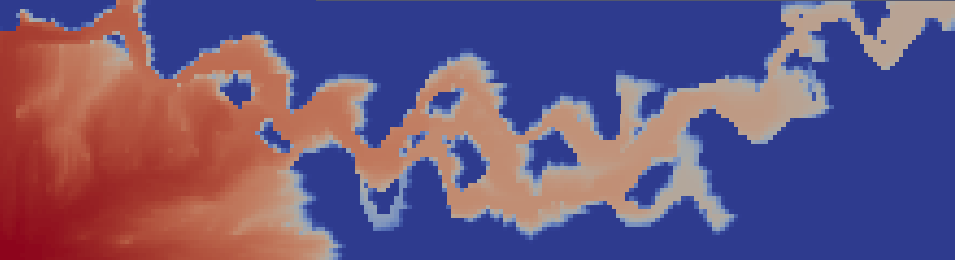
\includegraphics[width=\textwidth]{figures/saturation_upperness_layer-35.png}
\caption{Saturation at $T = \unit[30]{d}$}
\label{fig:saturation_upperness_layer-35}
\end{subfigure}
~
\begin{subfigure}{0.49\textwidth}
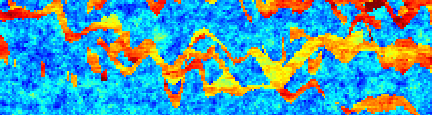
\includegraphics[width=\textwidth]{figures/perm_upperness_layer-35.png}
\caption{Permeability}
\label{fig:perm_upperness_layer-35}
\end{subfigure}
\caption{}
\label{fig:upperness_layer-35}
\end{figure}

\begin{figure}[!ht]
\tikzsetnextfilename{spe10_iterations_perm_i_36_0_0_m_1_10_i_50_dt_1to30}
\begin{subfigure}[b]{0.49\textwidth} %%%%%%%%%%% M = 0.1 %%%%%%%%%%%%%%
\begin{tikzpicture}
    \pgfplotstablegetrowsof{datafiles/spe10-iterations-s-r-T-400-m-1-10-dim-10-10-60-220-perm-i-36-0-0-i-50.data}
    \pgfmathsetmacro\yfin{\pgfmathresult}
    \pgfmathsetmacro\yini{5}
    \begin{semilogyaxis}[
            width=0.97\textwidth,
            height=0.26\textheight,
            ymin=300000,
            ymax=15600000,
            xlabel={dt~[days]},
            ylabel={\#iterations},
            grid=major,
            skip coords between index={\yini}{\yfin}
            ]
        \addplot table[col sep=comma, trim cells=true,x=dt, y=iterations] {datafiles/spe10-iterations-s-r-T-400-m-1-10-dim-10-10-60-220-perm-i-36-0-0-i-50.data};
        \addplot table[col sep=comma, trim cells=true,x=dt, y=iterations] {datafiles/spe10-iterations-s-t-T-400-m-1-10-dim-10-10-60-220-perm-i-36-0-0-i-50.data};
        \addplot table[col sep=comma, trim cells=true,x=dt, y=iterations] {datafiles/spe10-iterations-s-a-T-400-m-1-10-dim-10-10-60-220-perm-i-36-0-0-i-50.data};
        \addplot table[col sep=comma, trim cells=true,x=dt, y=iterations] {datafiles/spe10-iterations-s-b-T-400-m-1-10-dim-10-10-60-220-perm-i-36-0-0-i-50.data};
        \addplot table[col sep=comma, trim cells=true,x=dt, y=iterations] {datafiles/spe10-iterations-s-i-T-400-m-1-10-dim-10-10-60-220-perm-i-36-0-0-i-50.data};
        \legend{RF,TR,TR*,B,R}
    \end{semilogyaxis}
\end{tikzpicture}%
\caption{$M =0.1$} \label{fig:spe10_iterations_perm_i_36_0_0_m_1_10_i_50_dt_1to30}
\end{subfigure}%
~
\tikzsetnextfilename{spe10_iterations_perm_i_36_0_0_m_1_10_i_50_dt_40to150}
\begin{subfigure}[b]{0.49\textwidth}
\begin{tikzpicture}
    \pgfplotstablegetrowsof{datafiles/spe10-iterations-s-r-T-400-m-1-10-dim-10-10-60-220-perm-i-36-0-0-i-50.data}
    \pgfmathsetmacro\yfin{5}
    \pgfmathsetmacro\yini{0}
    \begin{semilogyaxis}[
            width=0.97\textwidth,
            height=0.26\textheight,
            ymin=70000,
            ymax=1000000,
            xlabel={dt~[days]},
            ylabel={\#iterations},
            grid=major,
            skip coords between index={\yini}{\yfin}
            ]
        \addplot table[col sep=comma, trim cells=true,x=dt, y=iterations] {datafiles/spe10-iterations-s-r-T-400-m-1-10-dim-10-10-60-220-perm-i-36-0-0-i-50.data};
        \addplot table[col sep=comma, trim cells=true,x=dt, y=iterations] {datafiles/spe10-iterations-s-t-T-400-m-1-10-dim-10-10-60-220-perm-i-36-0-0-i-50.data};
        \addplot table[col sep=comma, trim cells=true,x=dt, y=iterations] {datafiles/spe10-iterations-s-a-T-400-m-1-10-dim-10-10-60-220-perm-i-36-0-0-i-50.data};
        \addplot table[col sep=comma, trim cells=true,x=dt, y=iterations] {datafiles/spe10-iterations-s-b-T-400-m-1-10-dim-10-10-60-220-perm-i-36-0-0-i-50.data};
        \addplot table[col sep=comma, trim cells=true,x=dt, y=iterations] {datafiles/spe10-iterations-s-i-T-400-m-1-10-dim-10-10-60-220-perm-i-36-0-0-i-50.data};
        %\legend{RF,TR,TR*,B,R}
    \end{semilogyaxis}
\end{tikzpicture}%
\caption{$M =0.1$} \label{fig:spe10_iterations_perm_i_36_0_0_m_1_10_i_50_dt_40to150}
\end{subfigure}%
\vspace{0.3cm} %%%%%%%%%%% M = 1 %%%%%%%%%%%%%%
\tikzsetnextfilename{spe10_iterations_perm_i_36_0_0_m_1_1_i_50_dt_1to30}
\begin{subfigure}[b]{0.49\textwidth}
\begin{tikzpicture}
    \pgfplotstablegetrowsof{datafiles/spe10-iterations-s-r-T-400-m-1-10-dim-10-10-60-220-perm-i-36-0-0-i-50.data}
    \pgfmathsetmacro\yfin{\pgfmathresult}
    \pgfmathsetmacro\yini{5}
    \begin{semilogyaxis}[
            width=0.97\textwidth,
            height=0.26\textheight,
            ymin=190000,
            ymax=11500000,
            xlabel={dt~[days]},
            ylabel={\#iterations},
            grid=major,
            skip coords between index={\yini}{\yfin}
            ]
         \addplot table[col sep=comma, trim cells=true,x=dt, y=iterations] {datafiles/spe10-iterations-s-r-T-400-m-1-1-dim-10-10-60-220-perm-i-36-0-0-i-50.data};
        \addplot table[col sep=comma, trim cells=true,x=dt, y=iterations] {datafiles/spe10-iterations-s-t-T-400-m-1-1-dim-10-10-60-220-perm-i-36-0-0-i-50.data};
        \addplot table[col sep=comma, trim cells=true,x=dt, y=iterations] {datafiles/spe10-iterations-s-a-T-400-m-1-1-dim-10-10-60-220-perm-i-36-0-0-i-50.data};
        \addplot table[col sep=comma, trim cells=true,x=dt, y=iterations] {datafiles/spe10-iterations-s-b-T-400-m-1-1-dim-10-10-60-220-perm-i-36-0-0-i-50.data};
        \addplot table[col sep=comma, trim cells=true,x=dt, y=iterations] {datafiles/spe10-iterations-s-i-T-400-m-1-1-dim-10-10-60-220-perm-i-36-0-0-i-50.data};
        \legend{RF,TR,TR*,B,R}
    \end{semilogyaxis}
\end{tikzpicture}%
\caption{$M =1$} \label{fig:spe10_iterations_perm_i_36_0_0_m_1_1_i_50_dt_1to30}
\end{subfigure}%
~
\tikzsetnextfilename{spe10_iterations_perm_i_36_0_0_m_1_1_i_50_dt_40to150}
\begin{subfigure}[b]{0.49\textwidth}
\begin{tikzpicture}
    \pgfplotstablegetrowsof{datafiles/spe10-iterations-s-r-T-400-m-1-10-dim-10-10-60-220-perm-i-36-0-0-i-50.data}
    \pgfmathsetmacro\yfin{5}
    \pgfmathsetmacro\yini{0}
    \begin{semilogyaxis}[
            width=0.97\textwidth,
            height=0.26\textheight,
            ymin=60000,
            ymax=1000000,
            xlabel={dt~[days]},
            ylabel={\#iterations},
            grid=major,
            skip coords between index={\yini}{\yfin}
            ]
         \addplot table[col sep=comma, trim cells=true,x=dt, y=iterations] {datafiles/spe10-iterations-s-r-T-400-m-1-1-dim-10-10-60-220-perm-i-36-0-0-i-50.data};
        \addplot table[col sep=comma, trim cells=true,x=dt, y=iterations] {datafiles/spe10-iterations-s-t-T-400-m-1-1-dim-10-10-60-220-perm-i-36-0-0-i-50.data};
        \addplot table[col sep=comma, trim cells=true,x=dt, y=iterations] {datafiles/spe10-iterations-s-a-T-400-m-1-1-dim-10-10-60-220-perm-i-36-0-0-i-50.data};
        \addplot table[col sep=comma, trim cells=true,x=dt, y=iterations] {datafiles/spe10-iterations-s-b-T-400-m-1-1-dim-10-10-60-220-perm-i-36-0-0-i-50.data};
        \addplot table[col sep=comma, trim cells=true,x=dt, y=iterations] {datafiles/spe10-iterations-s-i-T-400-m-1-1-dim-10-10-60-220-perm-i-36-0-0-i-50.data};
        %\legend{RF,TR,TR*,B,R}
    \end{semilogyaxis}
\end{tikzpicture}%
\caption{$M =1$} \label{fig:spe10_iterations_perm_i_36_0_0_m_1_1_i_50_dt_40to150}
\end{subfigure}%
\vspace{0.3cm} %%%%%%%%%%% M = 10 %%%%%%%%%%%%%%
\tikzsetnextfilename{spe10_iterations_perm_i_36_0_0_m_10_1_i_50_dt_1to30}
\begin{subfigure}[b]{0.49\textwidth}
\begin{tikzpicture}
    \pgfplotstablegetrowsof{datafiles/spe10-iterations-s-r-T-400-m-1-10-dim-10-10-60-220-perm-i-36-0-0-i-50.data}
    \pgfmathsetmacro\yfin{\pgfmathresult}
    \pgfmathsetmacro\yini{5}
    \begin{semilogyaxis}[
            width=0.97\textwidth,
            height=0.26\textheight,
            ymin=200000,
            ymax=10000000,
            xlabel={dt~[days]},
            ylabel={\#iterations},
            grid=major,
            skip coords between index={\yini}{\yfin}
            ]
         \addplot table[col sep=comma, trim cells=true,x=dt, y=iterations] {datafiles/spe10-iterations-s-r-T-400-m-10-1-dim-10-10-60-220-perm-i-36-0-0-i-50.data};
        \addplot table[col sep=comma, trim cells=true,x=dt, y=iterations] {datafiles/spe10-iterations-s-t-T-400-m-10-1-dim-10-10-60-220-perm-i-36-0-0-i-50.data};
        \addplot table[col sep=comma, trim cells=true,x=dt, y=iterations] {datafiles/spe10-iterations-s-a-T-400-m-10-1-dim-10-10-60-220-perm-i-36-0-0-i-50.data};
        \addplot table[col sep=comma, trim cells=true,x=dt, y=iterations] {datafiles/spe10-iterations-s-b-T-400-m-10-1-dim-10-10-60-220-perm-i-36-0-0-i-50.data};
        \addplot table[col sep=comma, trim cells=true,x=dt, y=iterations] {datafiles/spe10-iterations-s-i-T-400-m-10-1-dim-10-10-60-220-perm-i-36-0-0-i-50.data};
        \legend{RF,TR,TR*,B,R}
    \end{semilogyaxis}
\end{tikzpicture}%
\caption{$M =10$} \label{fig:spe10_iterations_perm_i_36_0_0_m_10_1_i_50_dt_1to30}
\end{subfigure}%
~
\tikzsetnextfilename{spe10_iterations_perm_i_36_0_0_m_10_1_i_50_dt_40to150}
\begin{subfigure}[b]{0.49\textwidth}
\begin{tikzpicture}
    \pgfplotstablegetrowsof{datafiles/spe10-iterations-s-r-T-400-m-1-10-dim-10-10-60-220-perm-i-36-0-0-i-50.data}
    \pgfmathsetmacro\yfin{5}
    \pgfmathsetmacro\yini{0}
    \begin{semilogyaxis}[
            width=0.97\textwidth,
            height=0.26\textheight,
            ymin=64000,
            ymax=1000000,
            xlabel={dt~[days]},
            ylabel={\#iterations},
            grid=major,
            skip coords between index={\yini}{\yfin}
            ]
         \addplot table[col sep=comma, trim cells=true,x=dt, y=iterations] {datafiles/spe10-iterations-s-r-T-400-m-10-1-dim-10-10-60-220-perm-i-36-0-0-i-50.data};
        \addplot table[col sep=comma, trim cells=true,x=dt, y=iterations] {datafiles/spe10-iterations-s-t-T-400-m-10-1-dim-10-10-60-220-perm-i-36-0-0-i-50.data};
        \addplot table[col sep=comma, trim cells=true,x=dt, y=iterations] {datafiles/spe10-iterations-s-a-T-400-m-10-1-dim-10-10-60-220-perm-i-36-0-0-i-50.data};
        \addplot table[col sep=comma, trim cells=true,x=dt, y=iterations] {datafiles/spe10-iterations-s-b-T-400-m-10-1-dim-10-10-60-220-perm-i-36-0-0-i-50.data};
        \addplot table[col sep=comma, trim cells=true,x=dt, y=iterations] {datafiles/spe10-iterations-s-i-T-400-m-10-1-dim-10-10-60-220-perm-i-36-0-0-i-50.data};
        %\legend{RF,TR,TR*,B,R}
    \end{semilogyaxis}
\end{tikzpicture}%
\caption{$M =10$} \label{fig:spe10_iterations_perm_i_36_0_0_m_10_1_i_50_dt_40to150}
\end{subfigure}%
\caption{\#iterations used to solve case B, Section \ref{section:caseB}, for varying root finders, time steps and viscosity ratios.}
\label{fig:spe10_iterations_perm_i_36_0_0_i_50}
\end{figure}%
%
%\begin{figure}[!ht]
%\centering
%\tikzsetnextfilename{spe10_iterations_perm_i_36_0_0_m_1_10_i_50}
%\begin{subfigure}[b]{0.8\textwidth}
%\begin{tikzpicture}
%    \pgfplotstablegetrowsof{datafiles/spe10-iterations-s-r-T-400-m-1-10-dim-10-10-60-220-perm-i-36-0-0-i-50.data}
%    \pgfmathsetmacro\yfin{\pgfmathresult - 4}
%    \pgfmathsetmacro\yini{0}
%    \begin{semilogyaxis}[
%            width=0.97\textwidth,
%            height=0.26\textheight,
%            ymin=40000,
%            ymax=30000000,
%            xlabel={dt~[days]},
%            ylabel={\#iterations},
%            grid=major,
%            ]
%        \addplot table[col sep=comma, trim cells=true,x=dt, y=iterations] {datafiles/spe10-iterations-s-r-T-400-m-1-10-dim-10-10-60-220-perm-i-36-0-0-i-50.data};
%        \addplot table[col sep=comma, trim cells=true,x=dt, y=iterations] {datafiles/spe10-iterations-s-t-T-400-m-1-10-dim-10-10-60-220-perm-i-36-0-0-i-50.data};
%        \addplot table[col sep=comma, trim cells=true,x=dt, y=iterations] {datafiles/spe10-iterations-s-a-T-400-m-1-10-dim-10-10-60-220-perm-i-36-0-0-i-50.data};
%        \addplot table[col sep=comma, trim cells=true,x=dt, y=iterations] {datafiles/spe10-iterations-s-b-T-400-m-1-10-dim-10-10-60-220-perm-i-36-0-0-i-50.data};
%        \addplot table[col sep=comma, trim cells=true,x=dt, y=iterations] {datafiles/spe10-iterations-s-i-T-400-m-1-10-dim-10-10-60-220-perm-i-36-0-0-i-50.data};
%                %\addplot table[col sep=comma, trim cells=true,x=dt, y=iterations] {datafiles/spe10-iterations-s-g-T-400-m-1-10-dim-10-10-60-220-perm-i-36-0-0-i-50.data};
%        \legend{RF,TR,TR*,B,R}
%    \end{semilogyaxis}
%\end{tikzpicture}%
%\caption{$M =0.1$} \label{fig:spe10_iterations_perm_i_36_0_0_m_1_10_i_50}
%\end{subfigure}%
%\vspace{0.3cm}
%\centering
%\tikzsetnextfilename{spe10_iterations_perm_i_36_0_0_m_1_1_i_50}
%\begin{subfigure}[b]{0.8\textwidth}
%\begin{tikzpicture}
%    \begin{semilogyaxis}[
%            width=0.97\textwidth,
%            height=0.26\textheight,
%            ymin=40000,
%            ymax=30000000,
%            xlabel={dt~[days]},
%            ylabel={\#iterations},
%            grid=major,
%            ]
%         \addplot table[col sep=comma, trim cells=true,x=dt, y=iterations] {datafiles/spe10-iterations-s-r-T-400-m-1-1-dim-10-10-60-220-perm-i-36-0-0-i-50.data};
%        \addplot table[col sep=comma, trim cells=true,x=dt, y=iterations] {datafiles/spe10-iterations-s-t-T-400-m-1-1-dim-10-10-60-220-perm-i-36-0-0-i-50.data};
%        \addplot table[col sep=comma, trim cells=true,x=dt, y=iterations] {datafiles/spe10-iterations-s-a-T-400-m-1-1-dim-10-10-60-220-perm-i-36-0-0-i-50.data};
%        \addplot table[col sep=comma, trim cells=true,x=dt, y=iterations] {datafiles/spe10-iterations-s-b-T-400-m-1-1-dim-10-10-60-220-perm-i-36-0-0-i-50.data};
%        \addplot table[col sep=comma, trim cells=true,x=dt, y=iterations] {datafiles/spe10-iterations-s-i-T-400-m-1-1-dim-10-10-60-220-perm-i-36-0-0-i-50.data};
%                %\addplot table[col sep=comma, trim cells=true,x=dt, y=iterations] {datafiles/spe10-iterations-s-g-T-400-m-1-1-dim-10-10-60-220-perm-i-36-0-0-i-50.data};
%        \legend{RF,TR,TR*,B,R}
%    \end{semilogyaxis}
%\end{tikzpicture}%
%\caption{$M =1$} \label{fig:spe10_iterations_perm_i_36_0_0_m_1_1_i_50}
%\end{subfigure}%
%\vspace{0.3cm}
%\centering
%\tikzsetnextfilename{spe10_iterations_perm_i_36_0_0_m_10_1_i_50}
%\begin{subfigure}[b]{0.8\textwidth}
%\begin{tikzpicture}
%    \begin{semilogyaxis}[
%            width=0.97\textwidth,
%            height=0.26\textheight,
%            ymin=40000,
%            ymax=30000000,
%            xlabel={dt~[days]},
%            ylabel={\#iterations},
%            grid=major,
%            ]
%         \addplot table[col sep=comma, trim cells=true,x=dt, y=iterations] {datafiles/spe10-iterations-s-r-T-400-m-10-1-dim-10-10-60-220-perm-i-36-0-0-i-50.data};
%        \addplot table[col sep=comma, trim cells=true,x=dt, y=iterations] {datafiles/spe10-iterations-s-t-T-400-m-10-1-dim-10-10-60-220-perm-i-36-0-0-i-50.data};
%        \addplot table[col sep=comma, trim cells=true,x=dt, y=iterations] {datafiles/spe10-iterations-s-a-T-400-m-10-1-dim-10-10-60-220-perm-i-36-0-0-i-50.data};
%        \addplot table[col sep=comma, trim cells=true,x=dt, y=iterations] {datafiles/spe10-iterations-s-b-T-400-m-10-1-dim-10-10-60-220-perm-i-36-0-0-i-50.data};
%        \addplot table[col sep=comma, trim cells=true,x=dt, y=iterations] {datafiles/spe10-iterations-s-i-T-400-m-10-1-dim-10-10-60-220-perm-i-36-0-0-i-50.data};
%                %\addplot table[col sep=comma, trim cells=true,x=dt, y=iterations] {datafiles/spe10-iterations-s-g-T-400-m-10-1-dim-10-10-60-220-perm-i-36-0-0-i-50.data};
%        \legend{RF,TR,TR*,B,R}
%    \end{semilogyaxis}
%\end{tikzpicture}%
%\caption{$M =10$} \label{fig:spe10_iterations_perm_i_36_0_0_m_10_1_i_50}
%\end{subfigure}%
%\caption{\#iterations used to solve the Q5 problem, Section \ref{section:caseA}, for varying root finders, time steps and viscosity ratios.}
%\label{fig:spe10_iterations_perm_i_36_0_0_i_50}
%\end{figure}
\begin{figure}[!ht]
\centering
\tikzsetnextfilename{spe10_cputime_perm_i_36_0_0_m_1_10_i_50}
\begin{subfigure}[b]{0.8\textwidth}
\begin{tikzpicture}
    \begin{semilogyaxis}[
            width=0.97\textwidth,
            height=0.26\textheight,
            xlabel={dt~[d]},
            ylabel={CPU time~[s]},
            grid=both,
            ]
        \addplot table[col sep=comma, trim cells=true,x=dt, y=cputime] {datafiles/spe10-cputvsdt-s-r-T-400-m-1-10-dim-10-10-60-220-perm-i-36-0-0-i-50.data};
        \addplot table[col sep=comma, trim cells=true,x=dt, y=cputime] {datafiles/spe10-cputvsdt-s-t-T-400-m-1-10-dim-10-10-60-220-perm-i-36-0-0-i-50.data};
        \addplot table[col sep=comma, trim cells=true,x=dt, y=cputime] {datafiles/spe10-cputvsdt-s-a-T-400-m-1-10-dim-10-10-60-220-perm-i-36-0-0-i-50.data};
        \addplot table[col sep=comma, trim cells=true,x=dt, y=cputime] {datafiles/spe10-cputvsdt-s-b-T-400-m-1-10-dim-10-10-60-220-perm-i-36-0-0-i-50.data};
        \addplot table[col sep=comma, trim cells=true,x=dt, y=cputime] {datafiles/spe10-cputvsdt-s-i-T-400-m-1-10-dim-10-10-60-220-perm-i-36-0-0-i-50.data};
        \legend{RF,TR,TR*,B,R}
    \end{semilogyaxis}
\end{tikzpicture}%
\caption{$M =0.1$} \label{fig:spe10_cputime_perm_i_36_0_0_m_1_10_i_50}
\end{subfigure}%
\vspace{0.3cm}
\centering
\tikzsetnextfilename{spe10_cputime_perm_i_36_0_0_m_1_1_i_50}
\begin{subfigure}[b]{0.8\textwidth}
\begin{tikzpicture}
    \begin{semilogyaxis}[
            width=0.97\textwidth,
            height=0.26\textheight,
            xlabel={dt~[d]},
            ylabel={CPU time~[s]},
            grid=both,
            ]
         \addplot table[col sep=comma, trim cells=true,x=dt, y=cputime] {datafiles/spe10-cputvsdt-s-r-T-400-m-1-1-dim-10-10-60-220-perm-i-36-0-0-i-50.data};
        \addplot table[col sep=comma, trim cells=true,x=dt, y=cputime] {datafiles/spe10-cputvsdt-s-t-T-400-m-1-1-dim-10-10-60-220-perm-i-36-0-0-i-50.data};
        \addplot table[col sep=comma, trim cells=true,x=dt, y=cputime] {datafiles/spe10-cputvsdt-s-a-T-400-m-1-1-dim-10-10-60-220-perm-i-36-0-0-i-50.data};
        \addplot table[col sep=comma, trim cells=true,x=dt, y=cputime] {datafiles/spe10-cputvsdt-s-b-T-400-m-1-1-dim-10-10-60-220-perm-i-36-0-0-i-50.data};
        \addplot table[col sep=comma, trim cells=true,x=dt, y=cputime] {datafiles/spe10-cputvsdt-s-i-T-400-m-1-1-dim-10-10-60-220-perm-i-36-0-0-i-50.data};
        \legend{RF,TR,TR*,B,R}
    \end{semilogyaxis}
\end{tikzpicture}%
\caption{$M =1$} \label{fig:spe10_cputime_perm_i_36_0_0_m_1_1_i_50}
\end{subfigure}%
\vspace{0.3cm}
\centering
\tikzsetnextfilename{spe10_cputime_perm_i_36_0_0_m_10_1_i_50}
\begin{subfigure}[b]{0.8\textwidth}
\begin{tikzpicture}
    \begin{semilogyaxis}[
            width=0.97\textwidth,
            height=0.26\textheight,
            xlabel={dt~[d]},
            ylabel={CPU time~[s]},
            grid=both,
            ]
         \addplot table[col sep=comma, trim cells=true,x=dt, y=cputime] {datafiles/spe10-cputvsdt-s-r-T-400-m-10-1-dim-10-10-60-220-perm-i-36-0-0-i-50.data};
        \addplot table[col sep=comma, trim cells=true,x=dt, y=cputime] {datafiles/spe10-cputvsdt-s-t-T-400-m-10-1-dim-10-10-60-220-perm-i-36-0-0-i-50.data};
        \addplot table[col sep=comma, trim cells=true,x=dt, y=cputime] {datafiles/spe10-cputvsdt-s-a-T-400-m-10-1-dim-10-10-60-220-perm-i-36-0-0-i-50.data};
        \addplot table[col sep=comma, trim cells=true,x=dt, y=cputime] {datafiles/spe10-cputvsdt-s-b-T-400-m-10-1-dim-10-10-60-220-perm-i-36-0-0-i-50.data};
        \addplot table[col sep=comma, trim cells=true,x=dt, y=cputime] {datafiles/spe10-cputvsdt-s-i-T-400-m-10-1-dim-10-10-60-220-perm-i-36-0-0-i-50.data};
        \legend{RF,TR,TR*,B,R}
    \end{semilogyaxis}
\end{tikzpicture}%
\caption{$M =10$} \label{fig:spe10_cputime_perm_i_36_0_0_m_10_1_i_50}
\end{subfigure}%
\caption{CPU time used to solve case C, Section \ref{section:caseC}, for varying root finders, time steps and viscosity ratios.}
\label{fig:spe10_cputime_perm_i_36_0_0_i_50}
\end{figure}

\begin{figure}[!ht]
\centering
\tikzsetnextfilename{spe10_cputimetrans_perm_i_36_0_0_m_1_10_i_50}
\begin{subfigure}[b]{0.8\textwidth}
\begin{tikzpicture}
    \begin{semilogyaxis}[
            width=0.97\textwidth,
            height=0.26\textheight,
            xlabel={dt~[d]},
            ylabel={CPU time~[s]},
            grid=both,
            ]
        \addplot table[col sep=comma, trim cells=true,x=dt, y=cputime] {datafiles/spe10-cputransvsdt-s-r-T-400-m-1-10-dim-10-10-60-220-perm-i-36-0-0-i-50.data};
        \addplot table[col sep=comma, trim cells=true,x=dt, y=cputime] {datafiles/spe10-cputransvsdt-s-t-T-400-m-1-10-dim-10-10-60-220-perm-i-36-0-0-i-50.data};
        \addplot table[col sep=comma, trim cells=true,x=dt, y=cputime] {datafiles/spe10-cputransvsdt-s-a-T-400-m-1-10-dim-10-10-60-220-perm-i-36-0-0-i-50.data};
        \addplot table[col sep=comma, trim cells=true,x=dt, y=cputime] {datafiles/spe10-cputransvsdt-s-b-T-400-m-1-10-dim-10-10-60-220-perm-i-36-0-0-i-50.data};
        \addplot table[col sep=comma, trim cells=true,x=dt, y=cputime] {datafiles/spe10-cputransvsdt-s-i-T-400-m-1-10-dim-10-10-60-220-perm-i-36-0-0-i-50.data};                
        \legend{RF,TR,TR*,B,R}
    \end{semilogyaxis}
\end{tikzpicture}%
\caption{$M =0.1$} \label{fig:spe10_cputimetrans_perm_i_36_0_0_m_1_10_i_50}
\end{subfigure}%
\vspace{0.3cm}
\centering
\tikzsetnextfilename{spe10_cputimetrans_perm_i_36_0_0_m_1_1_i_50}	
\begin{subfigure}[b]{0.8\textwidth}
\begin{tikzpicture}
    \begin{semilogyaxis}[
            width=0.97\textwidth,
            height=0.26\textheight,
            xlabel={dt~[d]},
            ylabel={CPU time~[s]},
            grid=both,
            ]
         \addplot table[col sep=comma, trim cells=true,x=dt, y=cputime] {datafiles/spe10-cputransvsdt-s-r-T-400-m-1-1-dim-10-10-60-220-perm-i-36-0-0-i-50.data};
        \addplot table[col sep=comma, trim cells=true,x=dt, y=cputime] {datafiles/spe10-cputransvsdt-s-t-T-400-m-1-1-dim-10-10-60-220-perm-i-36-0-0-i-50.data};
        \addplot table[col sep=comma, trim cells=true,x=dt, y=cputime] {datafiles/spe10-cputransvsdt-s-a-T-400-m-1-1-dim-10-10-60-220-perm-i-36-0-0-i-50.data};
        \addplot table[col sep=comma, trim cells=true,x=dt, y=cputime] {datafiles/spe10-cputransvsdt-s-b-T-400-m-1-1-dim-10-10-60-220-perm-i-36-0-0-i-50.data};
        \addplot table[col sep=comma, trim cells=true,x=dt, y=cputime] {datafiles/spe10-cputransvsdt-s-i-T-400-m-1-1-dim-10-10-60-220-perm-i-36-0-0-i-50.data};
        \legend{RF,TR,TR*,B,R}
    \end{semilogyaxis}
\end{tikzpicture}%
\caption{$M =1$} \label{fig:spe10_cputimetrans_perm_i_36_0_0_m_1_1_i_50}
\end{subfigure}%
\vspace{0.3cm}
\centering
\tikzsetnextfilename{spe10_cputimetrans_perm_i_36_0_0_m_10_1_i_50}
\begin{subfigure}[b]{0.8\textwidth}
\begin{tikzpicture}
    \begin{semilogyaxis}[
            width=0.97\textwidth,
            height=0.26\textheight,
            xlabel={dt~[d]},
            ylabel={CPU time~[s]},
            grid=both,
            ]
         \addplot table[col sep=comma, trim cells=true,x=dt, y=cputime] {datafiles/spe10-cputransvsdt-s-r-T-400-m-10-1-dim-10-10-60-220-perm-i-36-0-0-i-50.data};
        \addplot table[col sep=comma, trim cells=true,x=dt, y=cputime] {datafiles/spe10-cputransvsdt-s-t-T-400-m-10-1-dim-10-10-60-220-perm-i-36-0-0-i-50.data};
        \addplot table[col sep=comma, trim cells=true,x=dt, y=cputime] {datafiles/spe10-cputransvsdt-s-a-T-400-m-10-1-dim-10-10-60-220-perm-i-36-0-0-i-50.data};
        \addplot table[col sep=comma, trim cells=true,x=dt, y=cputime] {datafiles/spe10-cputransvsdt-s-b-T-400-m-10-1-dim-10-10-60-220-perm-i-36-0-0-i-50.data};
        \addplot table[col sep=comma, trim cells=true,x=dt, y=cputime] {datafiles/spe10-cputransvsdt-s-i-T-400-m-10-1-dim-10-10-60-220-perm-i-36-0-0-i-50.data};
        \legend{RF,TR,TR*,B,R}
    \end{semilogyaxis}
\end{tikzpicture}%
\caption{$M =10$} \label{fig:spe10_cputimetrans_perm_i_36_0_0_m_10_1_i_50}
\end{subfigure}%
\caption{CPU time used by the transport solver when solving case C, Section \ref{section:caseC}, for varying root finders, time steps and viscosity ratios.}
\label{fig:spe10_cputimetrans_perm_i_36_0_0_i_50}
\end{figure}

\clearpage
%%%%%%%%%%%%%%%% TARBERT - 3D %%%%%%%%%%%%%%%%%%%
\subsection{Case D: Tarbert 3D}
\label{section:caseD}

\todoinline{Permeability/saturation plot for Tarbert 3D}
\todoinline{Run Tarbert 3D with gravity - cputime}
\todoinline{Run Tarbert 3D with gravity - iterations}

\clearpage
%%%%%%%%%%%%%%%%  UPPER NESS - 3D %%%%%%%%%%%%%%%%%%%
\subsection{Case E: Upper Ness 3D}
\label{section:caseE}

\todoinline{Permeability/saturation plot for Upper Ness 3D}
\todoinline{Run Upper Ness 3D with gravity - cputime}
\todoinline{Run Upper Ness 3D with gravity - iterations}

\clearpage
%%%%%%%%%%%%%%%% CONVERGENCE TESTS %%%%%%%%%%%%%%%%%%
\section{Convergence Tests}
\label{section:numerical_results_convergence_tests}
The efficiency of the numerical methods in terms of convergence speed can highlight the properties of the numerical procedures. We again \todo{Comment briefly on the properties of the viscosity residual when it is introduced.} observe that the form of the viscosity dominated residual from Equation (\ref{eq:residual_two_phase_transport}) is determined by five parameters; the initial saturation in the cell, $S_V^{n}$, the time step to pore volume ratio $\tau = \frac{\Delta t}{m(V)\phi_V}$, the flux out of the cell $q_o$, the flux into the cell $q_i$, and finally the viscosity ratio $M$ as defined in Equation (\ref{eq:viscosity_ratio}), held constant at $M = 1$. Note that the cell saturation from the previous time step is used as initial guess for the root finders. Figures \ref{fig:conv_res_in_0_05_out_0_05} through \ref{fig:conv_res_in_0_5_out_0_8} shows a number of different convergence and residual plots obtained by varying these parameters. 

Figure \ref{fig:conv_res_in_0_05_out_0_05} is obtained with incoming flux at $\unitfrac[0.05]{m^3}{s}$ and outgoing flux at $\unitfrac[0.05]{m^3}{s}$. Note that $\tau = \unitfrac[6]{s}{m^3}$. Under the circumstances the residuals are fairly linear, and the initial guess $S_0$ is close to the root. The number of iterations for all tested root finders decreases when $S_0$ is increased. We also note that the Newton-like methods converge faster than the other methods. This plot indicates that for small flux values the initial guess strongly influences the residual bringing the root close to $S_0$. with a stronger effect for larger $S_0$. 

Setting the incoming flux to $\unitfrac[0.35]{m^3}{s}$ and the outgoing flux to $\unitfrac[0.35]{m^3}{s}$ we obtain Figure \ref{fig:conv_res_in_0_35_out_0_35}. The residual plots shown a stronger non-linear influence, a fact reflected in the increased iteration count. $S_0$ still influences the residual, but to a lesser extent. Again we observe that large initial guesses generally leads to a lower iteration count. The Newton-like method are, together with Ridders, the best performers.

Moving on the even larger flux values, we set the incoming flux to $\unitfrac[0.5]{m^3}{s}$ and the outgoing flux to $\unitfrac[0.8]{m^3}{s}$. Figure \ref{fig:conv_res_in_0_5_out_0_8} shows the resulting plots. The trend from the previous plots continues, in that the initial guess has less influence on the performance of the root finders, on average. Interesting exceptions are the Newton-like methods. They perform significantly better in terms of iteration count when the initial guess is close, in contrast with the other methods. We also note that the initial has very little influence on the position of the root.

\begin{figure}[!ht]
\centering
\begin{subfigure}[b]{0.49\textwidth}
\begin{tikzpicture}
    \begin{semilogyaxis}[
            width=0.97\textwidth,
            height=0.3\textheight,
            xlabel={\#steps},
            ylabel={error},
            grid=both,
            legend pos=south west,
            ]
        \addplot table[col sep=comma, trim cells=true,x=iter, y=y] {testcasedatafiles/convergence2-s-r-M-1_000000-dtpv-6_000000-in--0_050000-out-0_050000-s0-0_100000.data};
        \addplot table[col sep=comma, trim cells=true,x=iter, y=y] {testcasedatafiles/convergence2-s-t-M-1_000000-dtpv-6_000000-in--0_050000-out-0_050000-s0-0_100000.data};
        \addplot table[col sep=comma, trim cells=true,x=iter, y=y] {testcasedatafiles/convergence2-s-a-M-1_000000-dtpv-6_000000-in--0_050000-out-0_050000-s0-0_100000.data};
        \addplot table[col sep=comma, trim cells=true,x=iter, y=y] {testcasedatafiles/convergence2-s-b-M-1_000000-dtpv-6_000000-in--0_050000-out-0_050000-s0-0_100000.data};
        \addplot table[col sep=comma, trim cells=true,x=iter, y=y] {testcasedatafiles/convergence2-s-i-M-1_000000-dtpv-6_000000-in--0_050000-out-0_050000-s0-0_100000.data};
        \addplot table[col sep=comma, trim cells=true,x=iter, y=y] {testcasedatafiles/convergence2-s-g-M-1_000000-dtpv-6_000000-in--0_050000-out-0_050000-s0-0_100000.data};
        \legend{RF,TR,TR*,B,R,GN}
    \end{semilogyaxis}
\end{tikzpicture}%
\caption{$S_0 = 0.1$}
\label{fig:convergence_in_0_05_out_0_05_s0_0_1}
\end{subfigure}%
\begin{subfigure}[b]{0.49\textwidth}
\begin{tikzpicture}
    \begin{axis}[
            width=0.97\textwidth,
            height=0.3\textheight,
            xlabel={S~[d]},
            ylabel={R(S)},
            grid=both,
            legend pos=north west,
            ]
        \addplot table[mark=none, col sep=comma, trim cells=true,x=s, y=Rs] {testcasedatafiles/residual-convergence2-s-r-M-1_000000-dtpv-6_000000-in--0_050000-out-0_050000-s0-0_100000.data};
        \addplot table[mark=none, col sep=comma, trim cells=true,x=s, y=dRs] {testcasedatafiles/residual-convergence2-s-r-M-1_000000-dtpv-6_000000-in--0_050000-out-0_050000-s0-0_100000.data};
            \legend{$R(S)$,$\partial_S R(S)$}
    \end{axis}
\end{tikzpicture}%
\caption{$S_0 = 0.1$}
\label{fig:residual_in_0_05_out_0_05_s0_0_1}
\end{subfigure}%
\vspace{0.4cm}
\begin{subfigure}[b]{0.49\textwidth}
\begin{tikzpicture}
    \begin{semilogyaxis}[
            width=0.97\textwidth,
            height=0.3\textheight,
            xlabel={\#steps},
            ylabel={error},
            grid=both,
            legend pos=south west,
            ]
        \addplot table[col sep=comma, trim cells=true,x=iter, y=y] {testcasedatafiles/convergence2-s-r-M-1_000000-dtpv-6_000000-in--0_050000-out-0_050000-s0-0_500000.data};
        \addplot table[col sep=comma, trim cells=true,x=iter, y=y] {testcasedatafiles/convergence2-s-t-M-1_000000-dtpv-6_000000-in--0_050000-out-0_050000-s0-0_500000.data};
        \addplot table[col sep=comma, trim cells=true,x=iter, y=y] {testcasedatafiles/convergence2-s-a-M-1_000000-dtpv-6_000000-in--0_050000-out-0_050000-s0-0_500000.data};
        \addplot table[col sep=comma, trim cells=true,x=iter, y=y] {testcasedatafiles/convergence2-s-b-M-1_000000-dtpv-6_000000-in--0_050000-out-0_050000-s0-0_500000.data};
        \addplot table[col sep=comma, trim cells=true,x=iter, y=y] {testcasedatafiles/convergence2-s-i-M-1_000000-dtpv-6_000000-in--0_050000-out-0_050000-s0-0_500000.data};
        \addplot table[col sep=comma, trim cells=true,x=iter, y=y] {testcasedatafiles/convergence2-s-g-M-1_000000-dtpv-6_000000-in--0_050000-out-0_050000-s0-0_500000.data};
        \legend{RF,TR,TR*,B,R,GN}
    \end{semilogyaxis}
\end{tikzpicture}%
\caption{$S_0 = 0.5$}
\label{fig:convergence_in_0_05_out_0_05_s0_0_5}
\end{subfigure}%
\begin{subfigure}[b]{0.49\textwidth}
\begin{tikzpicture}
    \begin{axis}[
            width=0.97\textwidth,
            height=0.3\textheight,
            xlabel={S},
            ylabel={$R(S)$},
            grid=both,
            legend pos=north west,
            ]
        \addplot table[mark=none, col sep=comma, trim cells=true,x=s, y=Rs] {testcasedatafiles/residual-convergence2-s-r-M-1_000000-dtpv-6_000000-in--0_050000-out-0_050000-s0-0_500000.data};
        \addplot table[mark=none, col sep=comma, trim cells=true,x=s, y=dRs] {testcasedatafiles/residual-convergence2-s-r-M-1_000000-dtpv-6_000000-in--0_050000-out-0_050000-s0-0_500000.data};
            \legend{$R(S)$,$\partial_S R(S)$}
    \end{axis}
\end{tikzpicture}%
\caption{$S_0 = 0.5$}
\label{fig:residual_in_0_05_out_0_05_s0_0_5}
\end{subfigure}%
\vspace{0.4cm}
\begin{subfigure}[b]{0.49\textwidth}
\begin{tikzpicture}
    \begin{semilogyaxis}[
            width=0.97\textwidth,
            height=0.3\textheight,
            xlabel={\#steps},
            ylabel={error},
            grid=both,
            legend pos=south west,
            ]
        \addplot table[col sep=comma, trim cells=true,x=iter, y=y] {testcasedatafiles/convergence2-s-r-M-1_000000-dtpv-6_000000-in--0_050000-out-0_050000-s0-0_900000.data};
        \addplot table[col sep=comma, trim cells=true,x=iter, y=y] {testcasedatafiles/convergence2-s-t-M-1_000000-dtpv-6_000000-in--0_050000-out-0_050000-s0-0_900000.data};
        \addplot table[col sep=comma, trim cells=true,x=iter, y=y] {testcasedatafiles/convergence2-s-a-M-1_000000-dtpv-6_000000-in--0_050000-out-0_050000-s0-0_900000.data};
        \addplot table[col sep=comma, trim cells=true,x=iter, y=y] {testcasedatafiles/convergence2-s-b-M-1_000000-dtpv-6_000000-in--0_050000-out-0_050000-s0-0_900000.data};
        \addplot table[col sep=comma, trim cells=true,x=iter, y=y] {testcasedatafiles/convergence2-s-i-M-1_000000-dtpv-6_000000-in--0_050000-out-0_050000-s0-0_900000.data};
        \addplot table[col sep=comma, trim cells=true,x=iter, y=y] {testcasedatafiles/convergence2-s-g-M-1_000000-dtpv-6_000000-in--0_050000-out-0_050000-s0-0_900000.data};
        \legend{RF,TR,TR*,B,R,GN}
    \end{semilogyaxis}
\end{tikzpicture}%
\caption{$S_0 = 0.9$}
\label{fig:convergence_in_0_05_out_0_05_s0_0_9}
\end{subfigure}%
\begin{subfigure}[b]{0.49\textwidth}
\begin{tikzpicture}
    \begin{axis}[
            width=0.97\textwidth,
            height=0.3\textheight,
            xlabel={S},
            ylabel={$R(S)$},
            grid=both,
            legend pos=north west,
            ]
        \addplot table[mark=none, col sep=comma, trim cells=true,x=s, y=Rs] {testcasedatafiles/residual-convergence2-s-r-M-1_000000-dtpv-6_000000-in--0_050000-out-0_050000-s0-0_900000.data};
        \addplot table[mark=none, col sep=comma, trim cells=true,x=s, y=dRs] {testcasedatafiles/residual-convergence2-s-r-M-1_000000-dtpv-6_000000-in--0_050000-out-0_050000-s0-0_900000.data};
            \legend{$R(S)$,$\partial_S R(S)$}
    \end{axis}
\end{tikzpicture}%
\caption{$S_0 = 0.9$}
\label{fig:residual_in_0_05_out_0_05_s0_0_9}
\end{subfigure}%
\caption{M = 1, dtpv = 6, influx = -0.05, outflux = 0.05}
\label{fig:conv_res_in_0_05_out_0_05}
\end{figure}

\begin{figure}[!ht]
\centering
\begin{subfigure}[b]{0.49\textwidth}
\begin{tikzpicture}
    \begin{semilogyaxis}[
            width=0.97\textwidth,
            height=0.3\textheight,
            xlabel={\#steps},
            ylabel={error},
            grid=both,
            legend pos=south west,
            ]
        \addplot table[col sep=comma, trim cells=true,x=iter, y=y] {testcasedatafiles/convergence2-s-r-M-1_000000-dtpv-6_000000-in--0_350000-out-0_350000-s0-0_100000.data};
        \addplot table[col sep=comma, trim cells=true,x=iter, y=y] {testcasedatafiles/convergence2-s-t-M-1_000000-dtpv-6_000000-in--0_350000-out-0_350000-s0-0_100000.data};
        \addplot table[col sep=comma, trim cells=true,x=iter, y=y] {testcasedatafiles/convergence2-s-a-M-1_000000-dtpv-6_000000-in--0_350000-out-0_350000-s0-0_100000.data};
        \addplot table[col sep=comma, trim cells=true,x=iter, y=y] {testcasedatafiles/convergence2-s-b-M-1_000000-dtpv-6_000000-in--0_350000-out-0_350000-s0-0_100000.data};
        \addplot table[col sep=comma, trim cells=true,x=iter, y=y] {testcasedatafiles/convergence2-s-i-M-1_000000-dtpv-6_000000-in--0_350000-out-0_350000-s0-0_100000.data};
        \addplot table[col sep=comma, trim cells=true,x=iter, y=y] {testcasedatafiles/convergence2-s-g-M-1_000000-dtpv-6_000000-in--0_350000-out-0_350000-s0-0_100000.data};
        \legend{RF,TR,TR*,B,R,GN}
    \end{semilogyaxis}
\end{tikzpicture}%
\caption{$S_0 = 0.1$}
\label{fig:convergence_in_0_35_out_0_35_s0_0_1}
\end{subfigure}%
\begin{subfigure}[b]{0.49\textwidth}
\begin{tikzpicture}
    \begin{axis}[
            width=0.97\textwidth,
            height=0.3\textheight,
            xlabel={S},
            ylabel={$R(S)$},
            grid=both,
            legend pos=north west,
            ]
        \addplot table[mark=none, col sep=comma, trim cells=true,x=s, y=Rs] {testcasedatafiles/residual-convergence2-s-r-M-1_000000-dtpv-6_000000-in--0_350000-out-0_350000-s0-0_100000.data};
        \addplot table[mark=none, col sep=comma, trim cells=true,x=s, y=dRs] {testcasedatafiles/residual-convergence2-s-r-M-1_000000-dtpv-6_000000-in--0_350000-out-0_350000-s0-0_100000.data};
            \legend{$R(S)$,$\partial_S R(S)$}
    \end{axis}
\end{tikzpicture}%
\caption{$S_0 = 0.1$}
\label{fig:residual_in_0_35_out_0_35_s0_0_1}
\end{subfigure}%
\vspace{0.4cm}
\begin{subfigure}[b]{0.49\textwidth}
\begin{tikzpicture}
    \begin{semilogyaxis}[
            width=0.97\textwidth,
            height=0.3\textheight,
            xlabel={\#steps},
            ylabel={error},
            grid=both,
            legend pos=south west,
            ]
        \addplot table[col sep=comma, trim cells=true,x=iter, y=y] {testcasedatafiles/convergence2-s-r-M-1_000000-dtpv-6_000000-in--0_350000-out-0_350000-s0-0_500000.data};
        \addplot table[col sep=comma, trim cells=true,x=iter, y=y] {testcasedatafiles/convergence2-s-t-M-1_000000-dtpv-6_000000-in--0_350000-out-0_350000-s0-0_500000.data};
        \addplot table[col sep=comma, trim cells=true,x=iter, y=y] {testcasedatafiles/convergence2-s-a-M-1_000000-dtpv-6_000000-in--0_350000-out-0_350000-s0-0_500000.data};
        \addplot table[col sep=comma, trim cells=true,x=iter, y=y] {testcasedatafiles/convergence2-s-b-M-1_000000-dtpv-6_000000-in--0_350000-out-0_350000-s0-0_500000.data};
        \addplot table[col sep=comma, trim cells=true,x=iter, y=y] {testcasedatafiles/convergence2-s-i-M-1_000000-dtpv-6_000000-in--0_350000-out-0_350000-s0-0_500000.data};
        \addplot table[col sep=comma, trim cells=true,x=iter, y=y] {testcasedatafiles/convergence2-s-g-M-1_000000-dtpv-6_000000-in--0_350000-out-0_350000-s0-0_500000.data};
        \legend{RF,TR,TR*,B,R,GN}
    \end{semilogyaxis}
\end{tikzpicture}%
\caption{$S_0 = 0.5$}
\label{fig:convergence_in_0_35_out_0_35_s0_0_5}
\end{subfigure}%
\begin{subfigure}[b]{0.49\textwidth}
\begin{tikzpicture}
    \begin{axis}[
            width=0.97\textwidth,
            height=0.3\textheight,
            xlabel={S},
            ylabel={$R(S)$},
            grid=both,
            legend pos=north west,
            ]
        \addplot table[mark=none, col sep=comma, trim cells=true,x=s, y=Rs] {testcasedatafiles/residual-convergence2-s-r-M-1_000000-dtpv-6_000000-in--0_350000-out-0_350000-s0-0_500000.data};
        \addplot table[mark=none, col sep=comma, trim cells=true,x=s, y=dRs] {testcasedatafiles/residual-convergence2-s-r-M-1_000000-dtpv-6_000000-in--0_350000-out-0_350000-s0-0_500000.data};
            \legend{$R(S)$,$\partial_S R(S)$}
    \end{axis}
\end{tikzpicture}%
\caption{$S_0 = 0.5$}
\label{fig:residual_in_0_35_out_0_35_s0_0_5}
\end{subfigure}%
\vspace{0.4cm}
\begin{subfigure}[b]{0.49\textwidth}
\begin{tikzpicture}
    \begin{semilogyaxis}[
            width=0.97\textwidth,
            height=0.3\textheight,
            xlabel={\#steps},
            ylabel={error},
            grid=both,
            legend pos=south west,
            ]
        \addplot table[col sep=comma, trim cells=true,x=iter, y=y] {testcasedatafiles/convergence2-s-r-M-1_000000-dtpv-6_000000-in--0_350000-out-0_350000-s0-0_900000.data};
        \addplot table[col sep=comma, trim cells=true,x=iter, y=y] {testcasedatafiles/convergence2-s-t-M-1_000000-dtpv-6_000000-in--0_350000-out-0_350000-s0-0_900000.data};
        \addplot table[col sep=comma, trim cells=true,x=iter, y=y] {testcasedatafiles/convergence2-s-a-M-1_000000-dtpv-6_000000-in--0_350000-out-0_350000-s0-0_900000.data};
        \addplot table[col sep=comma, trim cells=true,x=iter, y=y] {testcasedatafiles/convergence2-s-b-M-1_000000-dtpv-6_000000-in--0_350000-out-0_350000-s0-0_900000.data};
        \addplot table[col sep=comma, trim cells=true,x=iter, y=y] {testcasedatafiles/convergence2-s-i-M-1_000000-dtpv-6_000000-in--0_350000-out-0_350000-s0-0_900000.data};
        \addplot table[col sep=comma, trim cells=true,x=iter, y=y] {testcasedatafiles/convergence2-s-g-M-1_000000-dtpv-6_000000-in--0_350000-out-0_350000-s0-0_900000.data};
        \legend{RF,TR,TR*,B,R,GN}
    \end{semilogyaxis}
\end{tikzpicture}%
\caption{$S_0 = 0.9$}
\label{fig:convergence_in_0_35_out_0_35_s0_0_9}
\end{subfigure}%
\begin{subfigure}[b]{0.49\textwidth}
\begin{tikzpicture}
    \begin{axis}[
            width=0.97\textwidth,
            height=0.3\textheight,
            xlabel={S},
            ylabel={$R(S)$},
            grid=both,
            legend pos=north west,
            ]
        \addplot table[mark=none, col sep=comma, trim cells=true,x=s, y=Rs] {testcasedatafiles/residual-convergence2-s-r-M-1_000000-dtpv-6_000000-in--0_350000-out-0_350000-s0-0_900000.data};
        \addplot table[mark=none, col sep=comma, trim cells=true,x=s, y=dRs] {testcasedatafiles/residual-convergence2-s-r-M-1_000000-dtpv-6_000000-in--0_350000-out-0_350000-s0-0_900000.data};
            \legend{$R(S)$,$\partial_S R(S)$}
    \end{axis}
\end{tikzpicture}%
\caption{$S_0 = 0.9$}
\label{fig:residual_in_0_35_out_0_35_s0_0_9}
\end{subfigure}%
\caption{M = 1, dtpv = 6, influx = -0.35, outflux = 0.35}
\label{fig:conv_res_in_0_35_out_0_35}
\end{figure}

\begin{figure}[!ht]
\centering
\begin{subfigure}[b]{0.49\textwidth}
\begin{tikzpicture}
    \begin{semilogyaxis}[
            width=0.97\textwidth,
            height=0.3\textheight,
            xlabel={\#steps},
            ylabel={error},
            grid=both,
            legend pos=south west
            ]
        \addplot table[col sep=comma, trim cells=true,x=iter, y=y] {testcasedatafiles/convergence2-s-r-M-1_000000-dtpv-6_000000-in--0_500000-out-0_800000-s0-0_100000.data};
        \addplot table[col sep=comma, trim cells=true,x=iter, y=y] {testcasedatafiles/convergence2-s-t-M-1_000000-dtpv-6_000000-in--0_500000-out-0_800000-s0-0_100000.data};
        \addplot table[col sep=comma, trim cells=true,x=iter, y=y] {testcasedatafiles/convergence2-s-a-M-1_000000-dtpv-6_000000-in--0_500000-out-0_800000-s0-0_100000.data};
        \addplot table[col sep=comma, trim cells=true,x=iter, y=y] {testcasedatafiles/convergence2-s-b-M-1_000000-dtpv-6_000000-in--0_500000-out-0_800000-s0-0_100000.data};
        \addplot table[col sep=comma, trim cells=true,x=iter, y=y] {testcasedatafiles/convergence2-s-i-M-1_000000-dtpv-6_000000-in--0_500000-out-0_800000-s0-0_100000.data};
        \addplot table[col sep=comma, trim cells=true,x=iter, y=y] {testcasedatafiles/convergence2-s-g-M-1_000000-dtpv-6_000000-in--0_500000-out-0_800000-s0-0_100000.data};
        \legend{RF,TR,TR*,B,R,GN}
    \end{semilogyaxis}
\end{tikzpicture}%
\caption{$S_0 = 0.1$}
\label{fig:convergence_in_0_5_out_0_8_s0_0_1}
\end{subfigure}%
\begin{subfigure}[b]{0.49\textwidth}
\begin{tikzpicture}
    \begin{axis}[
            width=0.97\textwidth,
            height=0.3\textheight,
            xlabel={S},
            ylabel={$R(S)$},
            grid=both,
            legend pos=north west,
            ]
        \addplot table[mark=none, col sep=comma, trim cells=true,x=s, y=Rs] {testcasedatafiles/residual-convergence2-s-r-M-1_000000-dtpv-6_000000-in--0_500000-out-0_800000-s0-0_100000.data};
        \addplot table[mark=none, col sep=comma, trim cells=true,x=s, y=dRs] {testcasedatafiles/residual-convergence2-s-r-M-1_000000-dtpv-6_000000-in--0_500000-out-0_800000-s0-0_100000.data};
            \legend{$R(S)$,$\partial_S R(S)$}
    \end{axis}
\end{tikzpicture}%
\caption{$S_0 = 0.1$}
\label{fig:residual_in_0_5_out_0_8_s0_0_1}
\end{subfigure}%
\vspace{0.4cm}
\begin{subfigure}[b]{0.49\textwidth}
\begin{tikzpicture}
    \begin{semilogyaxis}[
            width=0.97\textwidth,
            height=0.3\textheight,
            xlabel={\#steps},
            ylabel={error},
            grid=both,
            legend pos=south west
            ]
        \addplot table[col sep=comma, trim cells=true,x=iter, y=y] {testcasedatafiles/convergence2-s-r-M-1_000000-dtpv-6_000000-in--0_500000-out-0_800000-s0-0_500000.data};
        \addplot table[col sep=comma, trim cells=true,x=iter, y=y] {testcasedatafiles/convergence2-s-t-M-1_000000-dtpv-6_000000-in--0_500000-out-0_800000-s0-0_500000.data};
        \addplot table[col sep=comma, trim cells=true,x=iter, y=y] {testcasedatafiles/convergence2-s-a-M-1_000000-dtpv-6_000000-in--0_500000-out-0_800000-s0-0_500000.data};
        \addplot table[col sep=comma, trim cells=true,x=iter, y=y] {testcasedatafiles/convergence2-s-b-M-1_000000-dtpv-6_000000-in--0_500000-out-0_800000-s0-0_500000.data};
        \addplot table[col sep=comma, trim cells=true,x=iter, y=y] {testcasedatafiles/convergence2-s-i-M-1_000000-dtpv-6_000000-in--0_500000-out-0_800000-s0-0_500000.data};
        \addplot table[col sep=comma, trim cells=true,x=iter, y=y] {testcasedatafiles/convergence2-s-g-M-1_000000-dtpv-6_000000-in--0_500000-out-0_800000-s0-0_500000.data};
        \legend{RF,TR,TR*,B,R,GN}
    \end{semilogyaxis}
\end{tikzpicture}%
\caption{$S_0 = 0.5$}
\label{fig:convergence_in_0_5_out_0_8_s0_0_5}
\end{subfigure}%
\begin{subfigure}[b]{0.49\textwidth}
\begin{tikzpicture}
    \begin{axis}[
            width=0.97\textwidth,
            height=0.3\textheight,
            xlabel={S},
            ylabel={$R(S)$},
            grid=both,
            legend pos=north west,
            ]
        \addplot table[mark=none, col sep=comma, trim cells=true,x=s, y=Rs] {testcasedatafiles/residual-convergence2-s-r-M-1_000000-dtpv-6_000000-in--0_500000-out-0_800000-s0-0_500000.data};
        \addplot table[mark=none, col sep=comma, trim cells=true,x=s, y=dRs] {testcasedatafiles/residual-convergence2-s-r-M-1_000000-dtpv-6_000000-in--0_500000-out-0_800000-s0-0_500000.data};
            \legend{$R(S)$,$\partial_S R(S)$}
    \end{axis}
\end{tikzpicture}%
\caption{$S_0 = 0.5$}
\label{fig:residual_in_0_5_out_0_8_s0_0_5}
\end{subfigure}%
\vspace{0.4cm}
\begin{subfigure}[b]{0.49\textwidth}
\begin{tikzpicture}
    \begin{semilogyaxis}[
            width=0.97\textwidth,
            height=0.3\textheight,
            xlabel={\#steps},
            ylabel={error},
            grid=both,
            legend pos=south west
            ]
        \addplot table[col sep=comma, trim cells=true,x=iter, y=y] {testcasedatafiles/convergence2-s-r-M-1_000000-dtpv-6_000000-in--0_500000-out-0_800000-s0-0_900000.data};
        \addplot table[col sep=comma, trim cells=true,x=iter, y=y] {testcasedatafiles/convergence2-s-t-M-1_000000-dtpv-6_000000-in--0_500000-out-0_800000-s0-0_900000.data};
        \addplot table[col sep=comma, trim cells=true,x=iter, y=y] {testcasedatafiles/convergence2-s-a-M-1_000000-dtpv-6_000000-in--0_500000-out-0_800000-s0-0_900000.data};
        \addplot table[col sep=comma, trim cells=true,x=iter, y=y] {testcasedatafiles/convergence2-s-b-M-1_000000-dtpv-6_000000-in--0_500000-out-0_800000-s0-0_900000.data};
        \addplot table[col sep=comma, trim cells=true,x=iter, y=y] {testcasedatafiles/convergence2-s-i-M-1_000000-dtpv-6_000000-in--0_500000-out-0_800000-s0-0_900000.data};
        \addplot table[col sep=comma, trim cells=true,x=iter, y=y] {testcasedatafiles/convergence2-s-g-M-1_000000-dtpv-6_000000-in--0_500000-out-0_800000-s0-0_900000.data};
        \legend{RF,TR,TR*,B,R,GN}
    \end{semilogyaxis}
\end{tikzpicture}%
\caption{$S_0 = 0.9$}
\label{fig:convergence_in_0_5_out_0_8_s0_0_9}
\end{subfigure}%
\begin{subfigure}[b]{0.49\textwidth}
\begin{tikzpicture}
    \begin{axis}[
            width=0.97\textwidth,
            height=0.3\textheight,
            xlabel={S},
            ylabel={$R(S)$},
            grid=both,
            legend pos=north west,
            ]
        \addplot table[mark=none, col sep=comma, trim cells=true,x=s, y=Rs] {testcasedatafiles/residual-convergence2-s-r-M-1_000000-dtpv-6_000000-in--0_500000-out-0_800000-s0-0_900000.data};
        \addplot table[mark=none, col sep=comma, trim cells=true,x=s, y=dRs] {testcasedatafiles/residual-convergence2-s-r-M-1_000000-dtpv-6_000000-in--0_500000-out-0_800000-s0-0_900000.data};
            \legend{$R(S)$,$\partial_S R(S)$}
    \end{axis}
\end{tikzpicture}%
\caption{$S_0 = 0.9$}
\label{fig:residual_in_0_5_out_0_8_s0_0_9}
\end{subfigure}%
\caption{M = 1, dtpv = 6, influx = -0.5, outflux = 0.8}
\label{fig:conv_res_in_0_5_out_0_8}
\end{figure}

